%!TeX program = xelatex
\documentclass[12pt,hyperref,a4paper,UTF8]{ctexart}
\usepackage{zjureport}
\usepackage{graphicx}
\usepackage{epstopdf}
\usepackage{subfloat}
\usepackage{booktabs}
\usepackage{listings}


%%-------------------------------正文开始---------------------------%%
\begin{document}

%%-----------------------封面--------------------%%
\cover

%%------------------摘要-------------%%
%\begin{abstract}
%
%在此填写摘要内容
%
%\end{abstract}

\thispagestyle{empty} % 首页不显示页码

%%--------------------------目录页------------------------%%
\newpage
\begin{spacing}{2}
\tableofcontents
\end{spacing}
\thispagestyle{empty}
\paragraph{}
\newpage
%%------------------------正文页从这里开始-------------------%


%%可选择这里也放一个标题
\begin{center}
    \title{ \Huge \textbf{{不规则物体的转动惯量测定方法}}}
\end{center}
\par
\begin{center}
    \textbf{Pan,He,Zhou,Zhou}
\end{center}
\paragraph{}

\section{背景知识}
\subsection{理论背景}

转动惯量又称为惯性矩,是物体的固有属性,描述了其在转动过程中对角速度变化的抵抗能力。在力学中,转动惯量通常用公式$I=\int r^2\text dm$表示,其中$r$是质量元$\text dm$到旋转轴的距离。它不仅取决于物体的质量分布,还与旋转轴的位置密切相关,因此轴的位置对转动惯量测量具有重要意义。

转动惯量的测量通常利用角动量守恒定律和牛顿第二定律的旋转形式。根据角动量定理,当合外力矩作用在刚体上时,刚体的角加速度$\alpha$与外力矩$\tau$之间满足$\tau=I\alpha$。通过已知外力矩和角加速度,可以反推刚体的转动惯量。

转动惯量的测定并非容易的问题,尤其是针对形状不规则的物体或拼接体。因此,采用扭摆法、三线摆法或落体法等间接方法在转动惯量的测定中备受欢迎。

\subsubsection{扭摆法}

扭摆法是一种利用扭转振动测量物体转动惯量的经典方法,其理论原理基于单摆运动与刚体转动的结合。扭摆的基本结构由悬挂刚体的细长弹性丝或扭转弹簧组成,当刚体被轻微旋转后,系统会产生周期性的扭转振动。

1. 扭转振动的基本原理

当刚体绕扭丝的轴发生微小转动时,弹性扭丝会产生恢复力矩$\tau$来抵抗这种转动,恢复力矩与角位移$\theta$成正比,即:

$$ \tau = -k \theta $$

根据刚体转动的牛顿第二定律:

$$ \tau = I \alpha $$

$$ I \frac{d^2\theta}{dt^2} + k\theta = 0 $$

该方程描述了刚体绕固定轴的简谐振动,其振动周期$T$为:

$$T = 2\pi \sqrt{\frac{I}{k}}$$

2. 测量扭转刚度 

扭转刚度$k$是弹性丝的固有属性,与其材料、直径、长度等参数有关。在实验中,可以通过已知转动惯量的标准物体测量扭转刚度:

$$k = \frac{4\pi^2 I_{\text{标准}}}{T_{\text{标准}}^2}$$

3. 测量未知物体的转动惯量

将待测物体安装在扭丝上,测量其扭转振动的周期 。通过已知的$T$值,利用下式计算转动惯量:

$$I = \frac{k T^2}{4\pi^2}$$

4. 复合物体的转动惯量

如果测量系统由扭丝、标准物体和待测物体组成,总转动惯量为:

$$I_{\text{总}} = I_{\text{标准}} + I_{\text{待测}}$$

5. 误差分析

使用扭摆法测量转动惯量时,主要误差来源包括:

扭丝非线性恢复力矩导致的系统误差。

振动周期测量中的读数误差。

扭丝刚度$k$计算误差。

系统外界扰动对振动周期的影响。


通过多次测量取平均值、减小扭丝非线性效应及减小振幅等措施可以有效降低误差。

总结

扭摆法通过测量振动周期并结合扭转刚度来精确计算物体的转动惯量。其优点在于结构简单、实验精度高,适用于多种刚体转动惯量的测量。

\subsubsection{三线摆法}

三线摆法是一种测量物体转动惯量的实验方法,其特点是结构简单、测量精度高,广泛应用于实验力学中。三线摆通过悬挂系统产生扭转振动,通过测量振动周期,结合系统的几何和物理参数计算待测物体的转动惯量。

1. 三线摆的基本结构

三线摆由三个等长且均匀分布的细线(或金属丝)悬挂一个刚体构成。细线的另一端固定在支架上。系统绕通过刚体重心且与三线平面垂直的轴进行自由扭转振动。刚体的重心与三线摆系统的对称性和力学平衡性保证了振动的稳定性。

2. 振动原理

三线摆的运动是绕垂直于线摆平面轴的扭转振动,其振动由刚体的转动惯量$I$与细线的弹性扭转力共同决定。当刚体偏离平衡位置发生转动时,细线的扭转恢复力矩使其产生简谐振动。

恢复力矩

细线因扭转产生的恢复力矩$\tau$与角位移$\theta$成正比:

$$ \tau = -k_{\text{总}} \theta $$

$$ k_{\text{总}} = 3k $$

振动方程

根据牛顿第二定律的转动形式:

$$ \tau = I \alpha $$

$$ I \frac{d^2\theta}{dt^2} + k_{\text{总}} \theta = 0 $$

$$ T = 2\pi \sqrt{\frac{I}{k_{\text{总}}}} $$

3. 转动惯量的测量

通过测量系统的振动周期$T$,可以计算出刚体的转动惯量:

$$ I = \frac{k_{\text{总}} T^2}{4\pi^2} $$

4. 扭转刚度的测量

细线的单根扭转刚度$k$可通过已知转动惯量的标准物体测量。将标准物体与三线摆系统相连,测量振动周期$T$,根据公式:

$ k = \frac{4\pi^2 I_{\text{标准}}}{3T_{\text{标准}}^2} $

5. 三线摆的理论优势

平衡性高:三根等长细线均匀分布,使系统具有良好的对称性和稳定性。

振动纯粹性:由于刚体的重心位于三线构成的平面中心,系统主要以扭转振动为主,避免了多余的摆动。

误差小:相比单线摆法,三线摆对外界干扰(如空气阻力、晃动)的敏感性较低。


6. 实验误差分析

细线非理想弹性:细线的刚度可能不是常数,可能会随振幅变化。

周期测量误差:振动周期的测量精度会直接影响结果。

安装误差:细线的长度、分布不均会导致刚体不稳定。

空气阻力:空气阻力可能会影响振动的衰减和周期。


通过增加测量次数取平均值、减小振动幅度等措施,可以有效降低误差。

\subsubsection{落体法}

落体法的理论原理

落体法是一种通过自由下落过程中物体的运动特性来测量转动惯量的实验方法。该方法利用能量守恒定律或动力学方程,通过物体的下落加速度、角速度及相关几何参数计算转动惯量。

1. 实验装置

落体法通常由以下部分组成:

一个绕固定轴旋转的刚体(待测物体)。

一个通过细绳连接的配重块,细绳绕过刚体的圆柱部分。

一个测量配重块加速度或刚体角加速度的装置。


当配重块自由下落时,细绳对刚体产生一个力矩,刚体开始旋转,整个系统的运动遵循力学定律。

2. 理论基础

落体法的理论主要基于以下两个物理规律:

(1)牛顿第二定律

配重块的线性运动由牛顿第二定律描述:

$$ ma = mg - T $$

 $m$为配重块质量;

 $a$为配重块的加速度;

 $g$为重力加速度;

 $T$为细绳对配重块的拉力。


(2)刚体转动方程

刚体的转动由转动牛顿第二定律描述:

$$  \tau = I \alpha $$

 $\tau=T\cdot R$是作用在刚体上的力矩;

 $I$是待测刚体的转动惯量;

 $\alpha$是刚体的角加速度;

 $R$是细绳绕刚体圆柱部分的半径。


此外,配重块的线性加速度$a$与刚体的角加速度$\alpha$满足几何关系:

$$ a = R \alpha $$

3. 转动惯量的计算

结合以上三个公式:

1. 配重块的动力学方程:

$$ I = R^2 \left( \frac{m g - m a}{a} \right) $$

$m$为配重块质量;

$g$为重力加速度;

$a$为配重块的线性加速度;

$R$为绳子绕刚体圆柱的半径。


4. 测量步骤

(1) 测量几何参数:精确测量绳子绕刚体圆柱的半径$R$和配重块的质量$m$。
(2) 测量加速度:通过传感器或视频分析记录配重块下落的加速度$a$。
(3) 计算转动惯量:代入公式计算刚体的转动惯量。
$$ I=R^2(\frac{mg-ma}{a}) $$


5. 优点与误差分析

优点

简单高效:实验装置简单,加速度的测量易于实现。

理论清晰:利用基本的牛顿运动定律和几何关系,公式推导简单明了。


误差来源

摩擦力影响:轴承摩擦和空气阻力可能导致测量误差。

加速度测量误差:加速度的测量精度直接影响计算结果。

绳子质量忽略:假设绳子质量远小于配重块质量,这可能带来系统误差。

非理想刚体:刚体可能存在形变或不均匀质量分布。


总结

落体法通过结合配重块的线性运动与刚体的转动,利用简单的动力学方程精确测量转动惯量。该方法以其简洁性和高效性在物理实验中得到了广泛应用,同时对实验装置的摩擦等影响因素的校正是提高测量精度的重要环节。


\section{实验装置}
\subsection{硬件架构}
本实验中主要的器材包括扭摆法器材、三线摆法器材和落体法器材。

此外,我们还通过Blender建模,3D打印制造了质量与体积已知的标准元件。用于转动惯量的测定实验。

\subsection{软件架构}
采用Blender进行模拟,研究不规则物体与流体的转动性质。


\section{实验操作}
\subsection{扭摆法}
\subsubsection{实验方法}

为了使用扭摆法计算刚体的转动惯量,我们需要测算扭摆扭丝的回复力矩,那么我们就要测出它的扭转系数。
这时,我们先令加了载物盘的扭丝空转,读出其转动的周期$ T_0 $;
再将一个具有已知转动惯量$ I_{\text{标准}} $的的物体(“标准物体”)加在载物盘上,读出其转动的周期$ T_1 $。
由于$ T_0 $和$ T_1 $是在转动角度$ \Delta \theta $极小的情况下读出的,
因此可以视作扭摆做简谐运动,其周期与这一小偏角无关。根据前文提到的计算扭转系数的方法,
并取$ T_{\text{标准}}^2 = T_1^2 - T_0^2 $,
可得$ k = \frac{4\pi^2 I_{\text{标准}}}{T_1^2 - T_0^2} $

按照同样的原理,取下标准物体,安装待测的不规则物体,并引导其以一小角度做周期性转动。
测量不规则物体进行小角度摆动时的周期$ T_{\text{测量}} $。
由$ I = \frac{k T_{\text{测量}}^2}{4\pi^2} $,即可求得不规则物体的转动惯量。

在这里,我们采取传感器直接测量角速度-时间数据的方法获得原始数据,
然后使用逐差法计算每两个角速度最大值间经过的时间即可求得周期的值。

利用相同的方法,我们还可以测量包含液体的容器的转动惯量。
此时,液体在容器壁上施加一个变阻力。如果为这个运动绘制角速度-时间图像,由于阻力的作用,
图像的包络线可以由方程$ \omega = \omega_0 e^{- \frac{\beta}{w} w_0 t} \sqrt{1 - \frac{beta^2}{w^2}} $描述。

\subsubsection{实验步骤}

1. 校准仪器

(1) 将传感器重启以复位。这会消除传感器上一次记录时留下的累计误差。

(2) 将扭摆载物盘调节至水平。先拆卸载物盘。
调节扭摆三足上的定位螺丝,直到安装在扭摆臂上的水平仪显示水平为止。
此时,扭摆的转轴已经调至垂直于地面。
然后,将传感器安装在载物盘的边缘,再将载物盘安装在转轴上。
转动转轴并调节载物盘安装位置,使得载物盘旋转到任意位置时,传感器读出的$ z $偏角都为0为止。

2. 测量扭丝的扭转系数

(1) 计算标准物体的转动惯量$ I_{\text{标准}} $。

(2) 将传感器安装至载物盘中心。此时,传感器与载物盘共轴。

(3) 使载物盘转动一个微小的角度$ \theta $,再使其自然回复。从传感器上读出$ T_0 $。

(4) 将标准物体紧固在载物盘上。
使载物盘转动一个微小的角度$ \theta $,再使其自然回复。从传感器上读出$ T_1 $。

(5) 计算扭转系数$ k $。

3. 测量不规则物体的转动惯量

(1) 拆下标准物体,将待测物体紧固在载物盘上。
使载物盘转动一个微小的角度$ \theta $,再使其自然回复。从传感器上读出$ T_{\text{测量}} $。

(2) 计算不规则物体的转动惯量$ I $。

4. 测量液体的的转动惯量

(1) 计算容器的转动惯量。

(2) 称量空容器质量,再将容器装满待测液体,测量得到总质量,相减得到液体质量。
将按照待装液体的质量,将其当作刚体来计算其转动惯量,即是$ I_{\text{液体}} $。

(3) 向容器中注满液体,紧固在载物盘上。
使载物盘转动一个微小的角度$ \theta $,再使其自然回复。从传感器上读出$ T_{\text{满容器}} $。

(4) 将容器倾空,紧固在载物盘上。
使载物盘转动一个微小的角度$ \theta $,再使其自然回复。从传感器上读出$ T_{\text{空容器}} $。

(5) 根据$ T_{\text{满容器}} $和$ T_{\text{空容器}} $计算出$ I_{\text{满容器}} $和$ I_{\text{空容器}} $,
相减得到$ I_{\text{液体}}^{'} $。

(6) 比较$ I_{\text{液体}} $与$ I_{\text{液体}}^{'} $,分析二者不同的原因。

5. Blender建模制作动画可视化研究液体转动行为

\subsubsection{实验数据}

2. 测量扭丝的扭转系数

\begin{figure}[htbp]
    \centering
    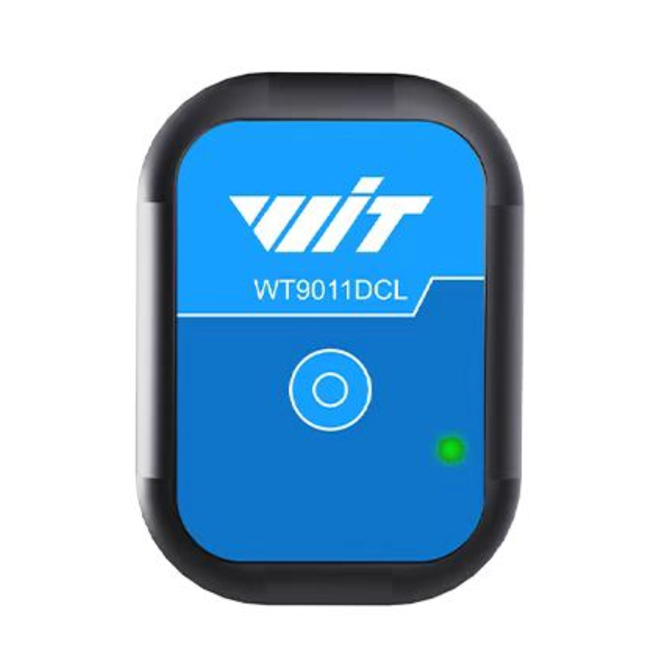
\includegraphics{sensor.eps}
    \caption{\text{实验采用的WT9011DCT型传感器}}
\end{figure}

在第一组实验中,我们取一圆柱状标准物体,
分别测量其上底面和下底面直径,取3次测量后平均,作为其直径;
取3次测量质量后平均,作为其质量。测量时,
我们设定传感器角速度采样间隔为0.1s,计算得的扭转系数如下:

\begin{table}[h!]
\centering
\begin{tabular}{|c|c|c|c|c|c|}
    \hline
      标准物体直径/$ 10^{-2} m $ & 标准物体质量/$kg$ & 转动惯量/$kg·m^2$ & $T_0$/$s$ & $T_1$/$s$ & $k$/$kg·m^2/s^2$\\
    \hline
      9.946 & 0.713 & $\text{8.817} \times \text{10}^{\text{-4}}$ & 0.633 & 1.033 & $\text{5.223} \times \text{10}^{\text{-5}}$ \\
    \hline
\end{tabular}
\caption{测量扭丝的扭转系数 - $ \Delta \text{t} = \text{0.1s} $}
\end{table}

在旋转液体转动惯量的测量实验中,我们通过设定传感器角速度采样间隔为0.001s,
对周期的精度作了修正。
通过排除传感器读出时间-角速度数据的前几组(此时,角度较大,不能视作简谐运动);
以及最后几组(此时,体系回到平衡位置附近,角速度已经不能视作恒定),
我们对周期数据作了修正。

\begin{table}[h!]
\centering
\begin{tabular}{|c|c|c|c|c|c|}
    \hline
        标准物体直径/$ 10^{-2} m $ & 标准物体质量/$kg$ & 转动惯量/$kg·m^2$ & $T_0$/$s$ & $T_1$/$s$ & $k$/$kg·m^2/s^2$\\
    \hline
        9.997 & 0.713 & $\text{2.215} \times \text{10}^{\text{-4}}$ & 0.627 & 1.488 & $\text{4.806} \times \text{10}^{\text{-5}}$ \\
    \hline
\end{tabular}
\caption{测量扭丝的扭转系数 - $ \Delta \text{t} = \text{0.1s} $}
\end{table}

3. 测量不规则物体的转动惯量

我们选取一个鼠标作为待测量的物体。为了确定其重心在轴线上,
我们将其凸起的背面朝下,倒置在载物盘上,支点放在轴心上。待鼠标稳定后,其重心恰在轴线的延长线上。
将双面胶贴在支点的位置,再将其固定到载物盘上。

\begin{figure}[htbp]
    \centering
    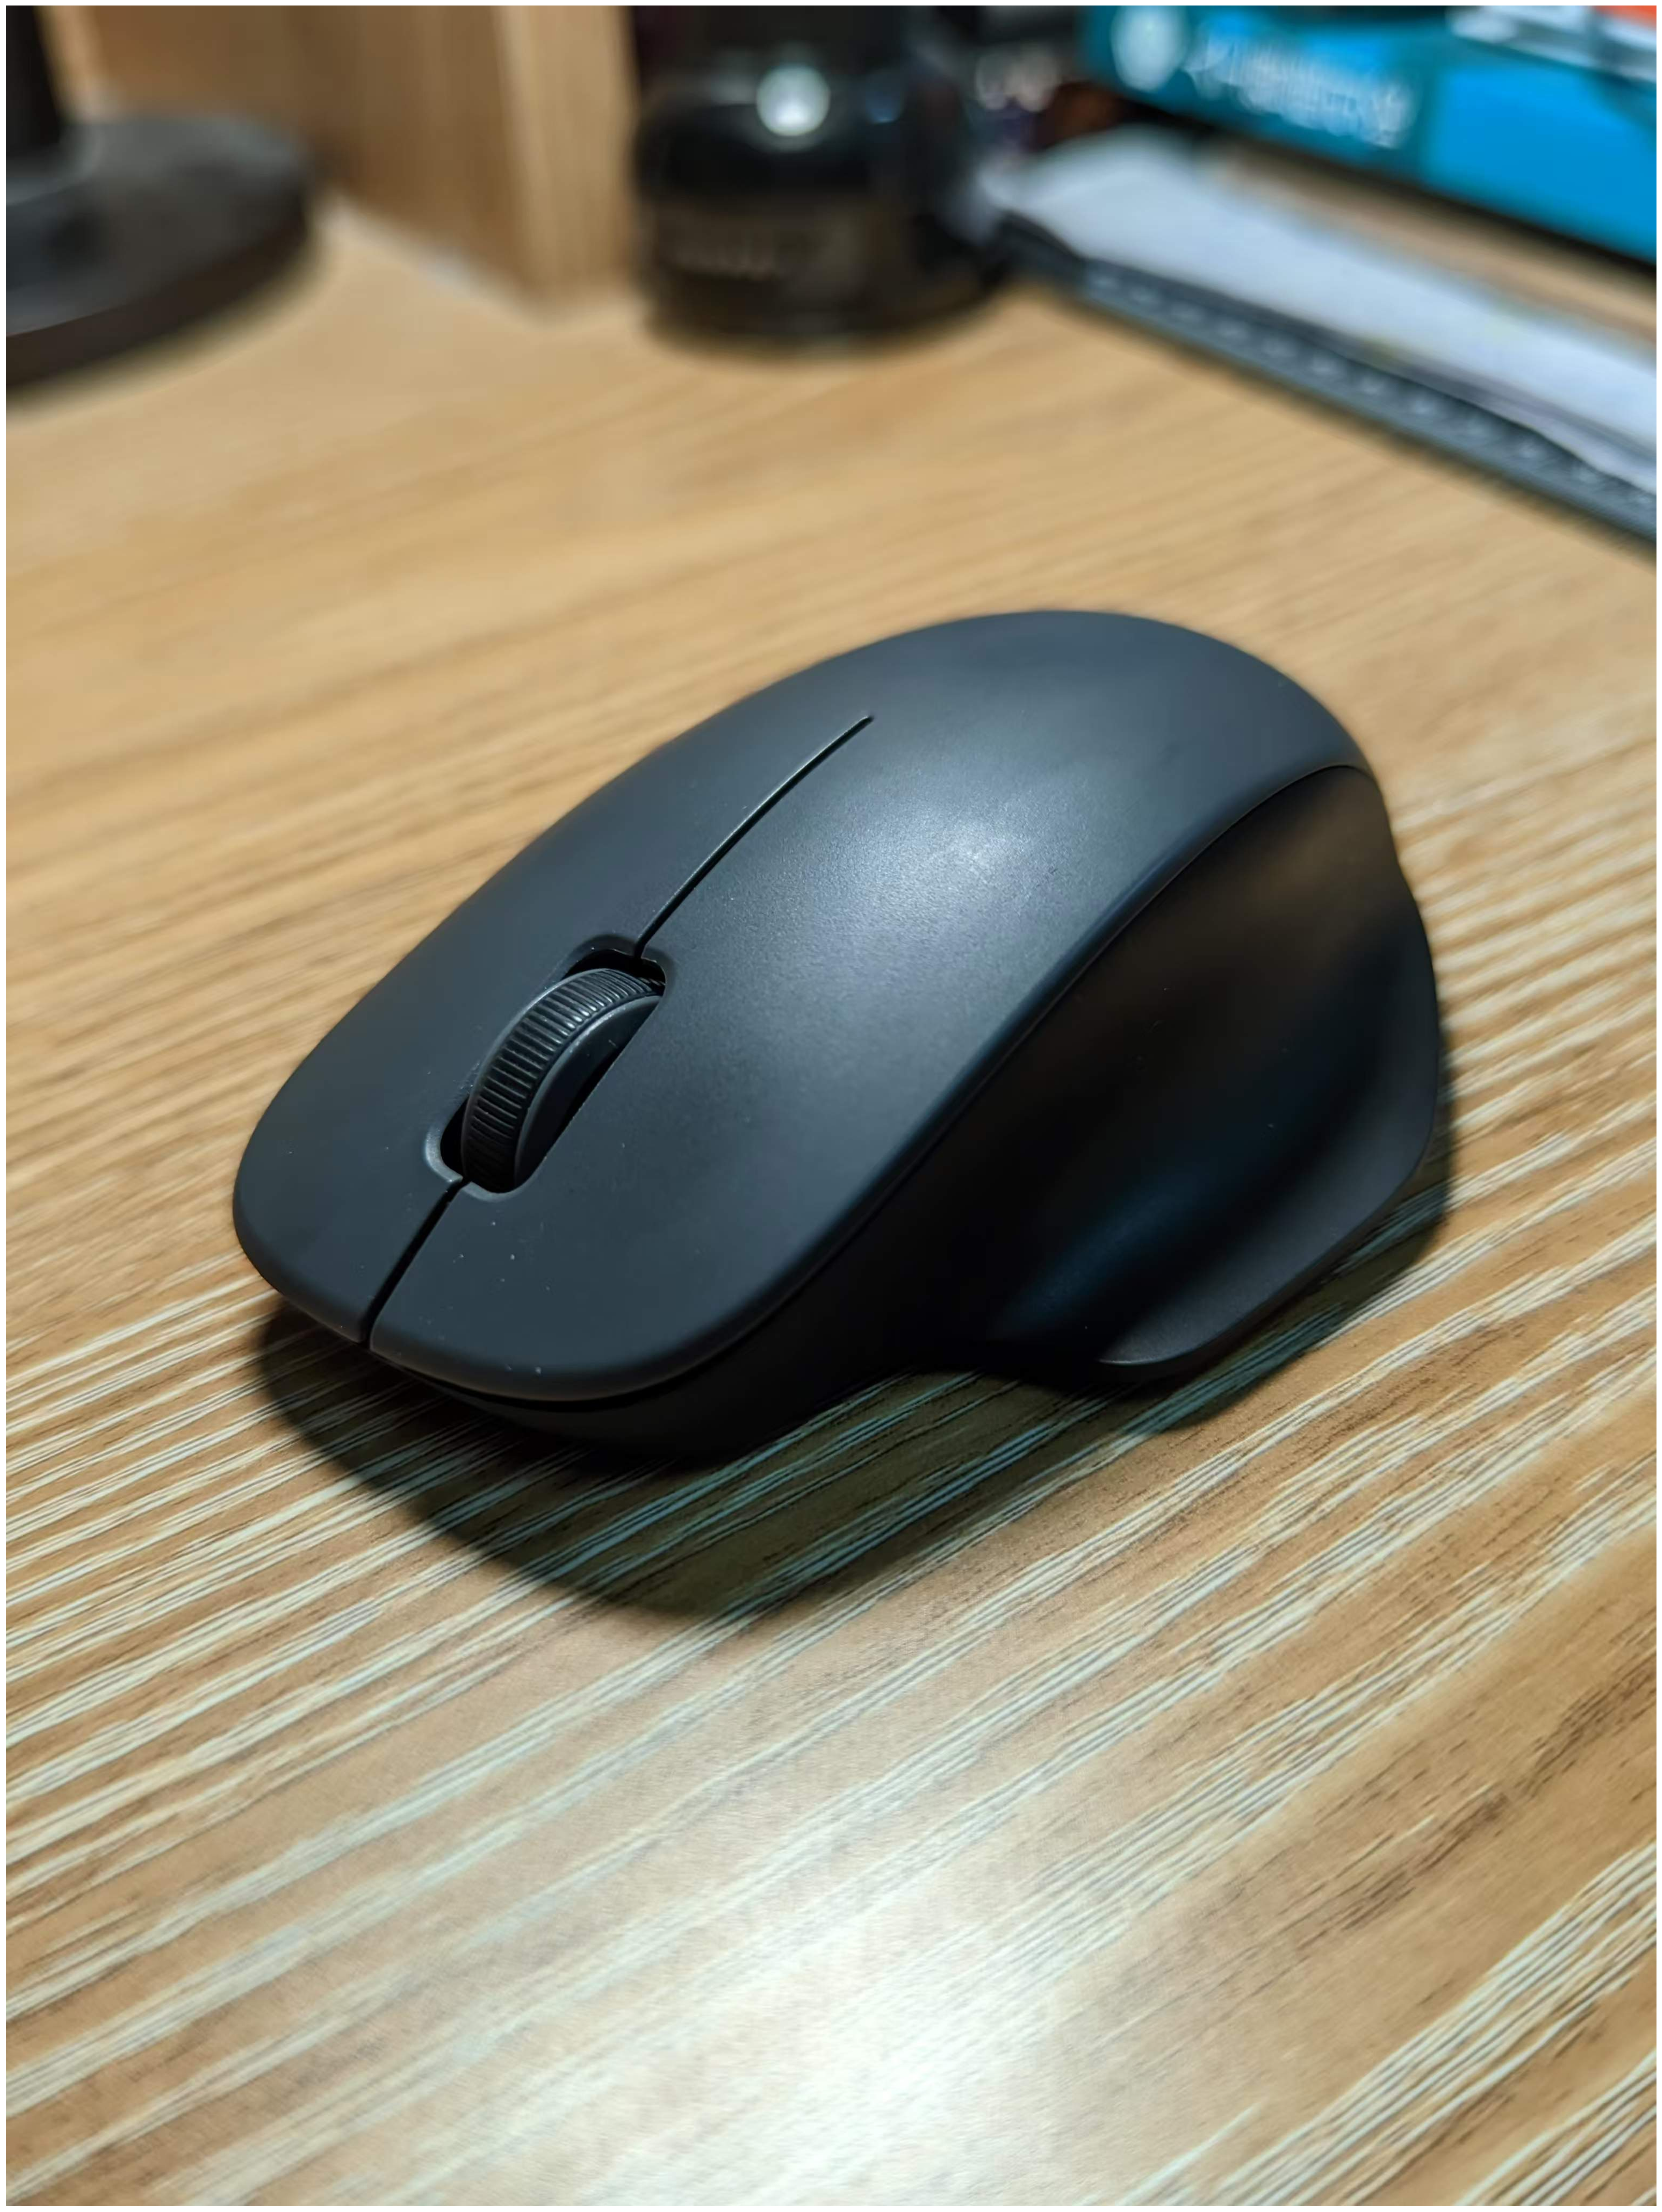
\includegraphics{mouse.eps}
    \caption{\text{待测量的物体}}
\end{figure}

在测量不规则物体的转动惯量时,我们设置传感器采样间隔为0.001s。
我们记录了转动开始后若干个周期的长度,逐差法得到单周期长,记录如下:

\begin{table}[h!]
\centering
\begin{tabular}{|c|c|c|c|c|c|c|c|c|c|c|c|}
    \hline
        达到最大角速度的时刻/$s$ & 39.731 & 40.579 & 41.411 & 42.282 & 43.150 & 43.989 & 44.831 & 45.728 & 46.573 & 47.411 & 48.250 \\
    \hline
        $ \Delta t $/$s$ & 0.848 & 0.832 & 0.871 & 0.868 & 0.839 & 0.842 & 0.897 & 0.845 & 0.838 & 0.839 & / \\
    \hline
        $ T $/$s$ & 0.852 & / & / & / & / & / & / & / & / & / & / \\
    \hline
        $ I $/$ kg·m^2 $ & $ \text{9.602} \times \text{10}^\text{-7} $ & / & / & / & / & / & / & / & / & / & / \\
    \hline
\end{tabular}
\caption{逐差法测量不规则物体转动周期及其转动惯量}
\end{table}

注:此实验取$ k = \text{5.223} \times \text{10}^{\text{-5}} $

4. 测量液体的的转动惯量

我们先按照前述理论计算旋转液体的转动惯量。
由于液体加满容器,其液面高度恒定,转动时不随角速度和半径变化,液体高度$h$为一常数$H$。
根据公式:

$$ I = \rho \int{2 \pi}{0} \int{R}{0} \int{H}{0} r^3 \text{d}z \text{d}r \text{d}\theta 
    &= \rho · 2\pi · H · \frac{R^4}{4} $$

以及观察数据:

\begin{figure}[htbp]
    \centering
    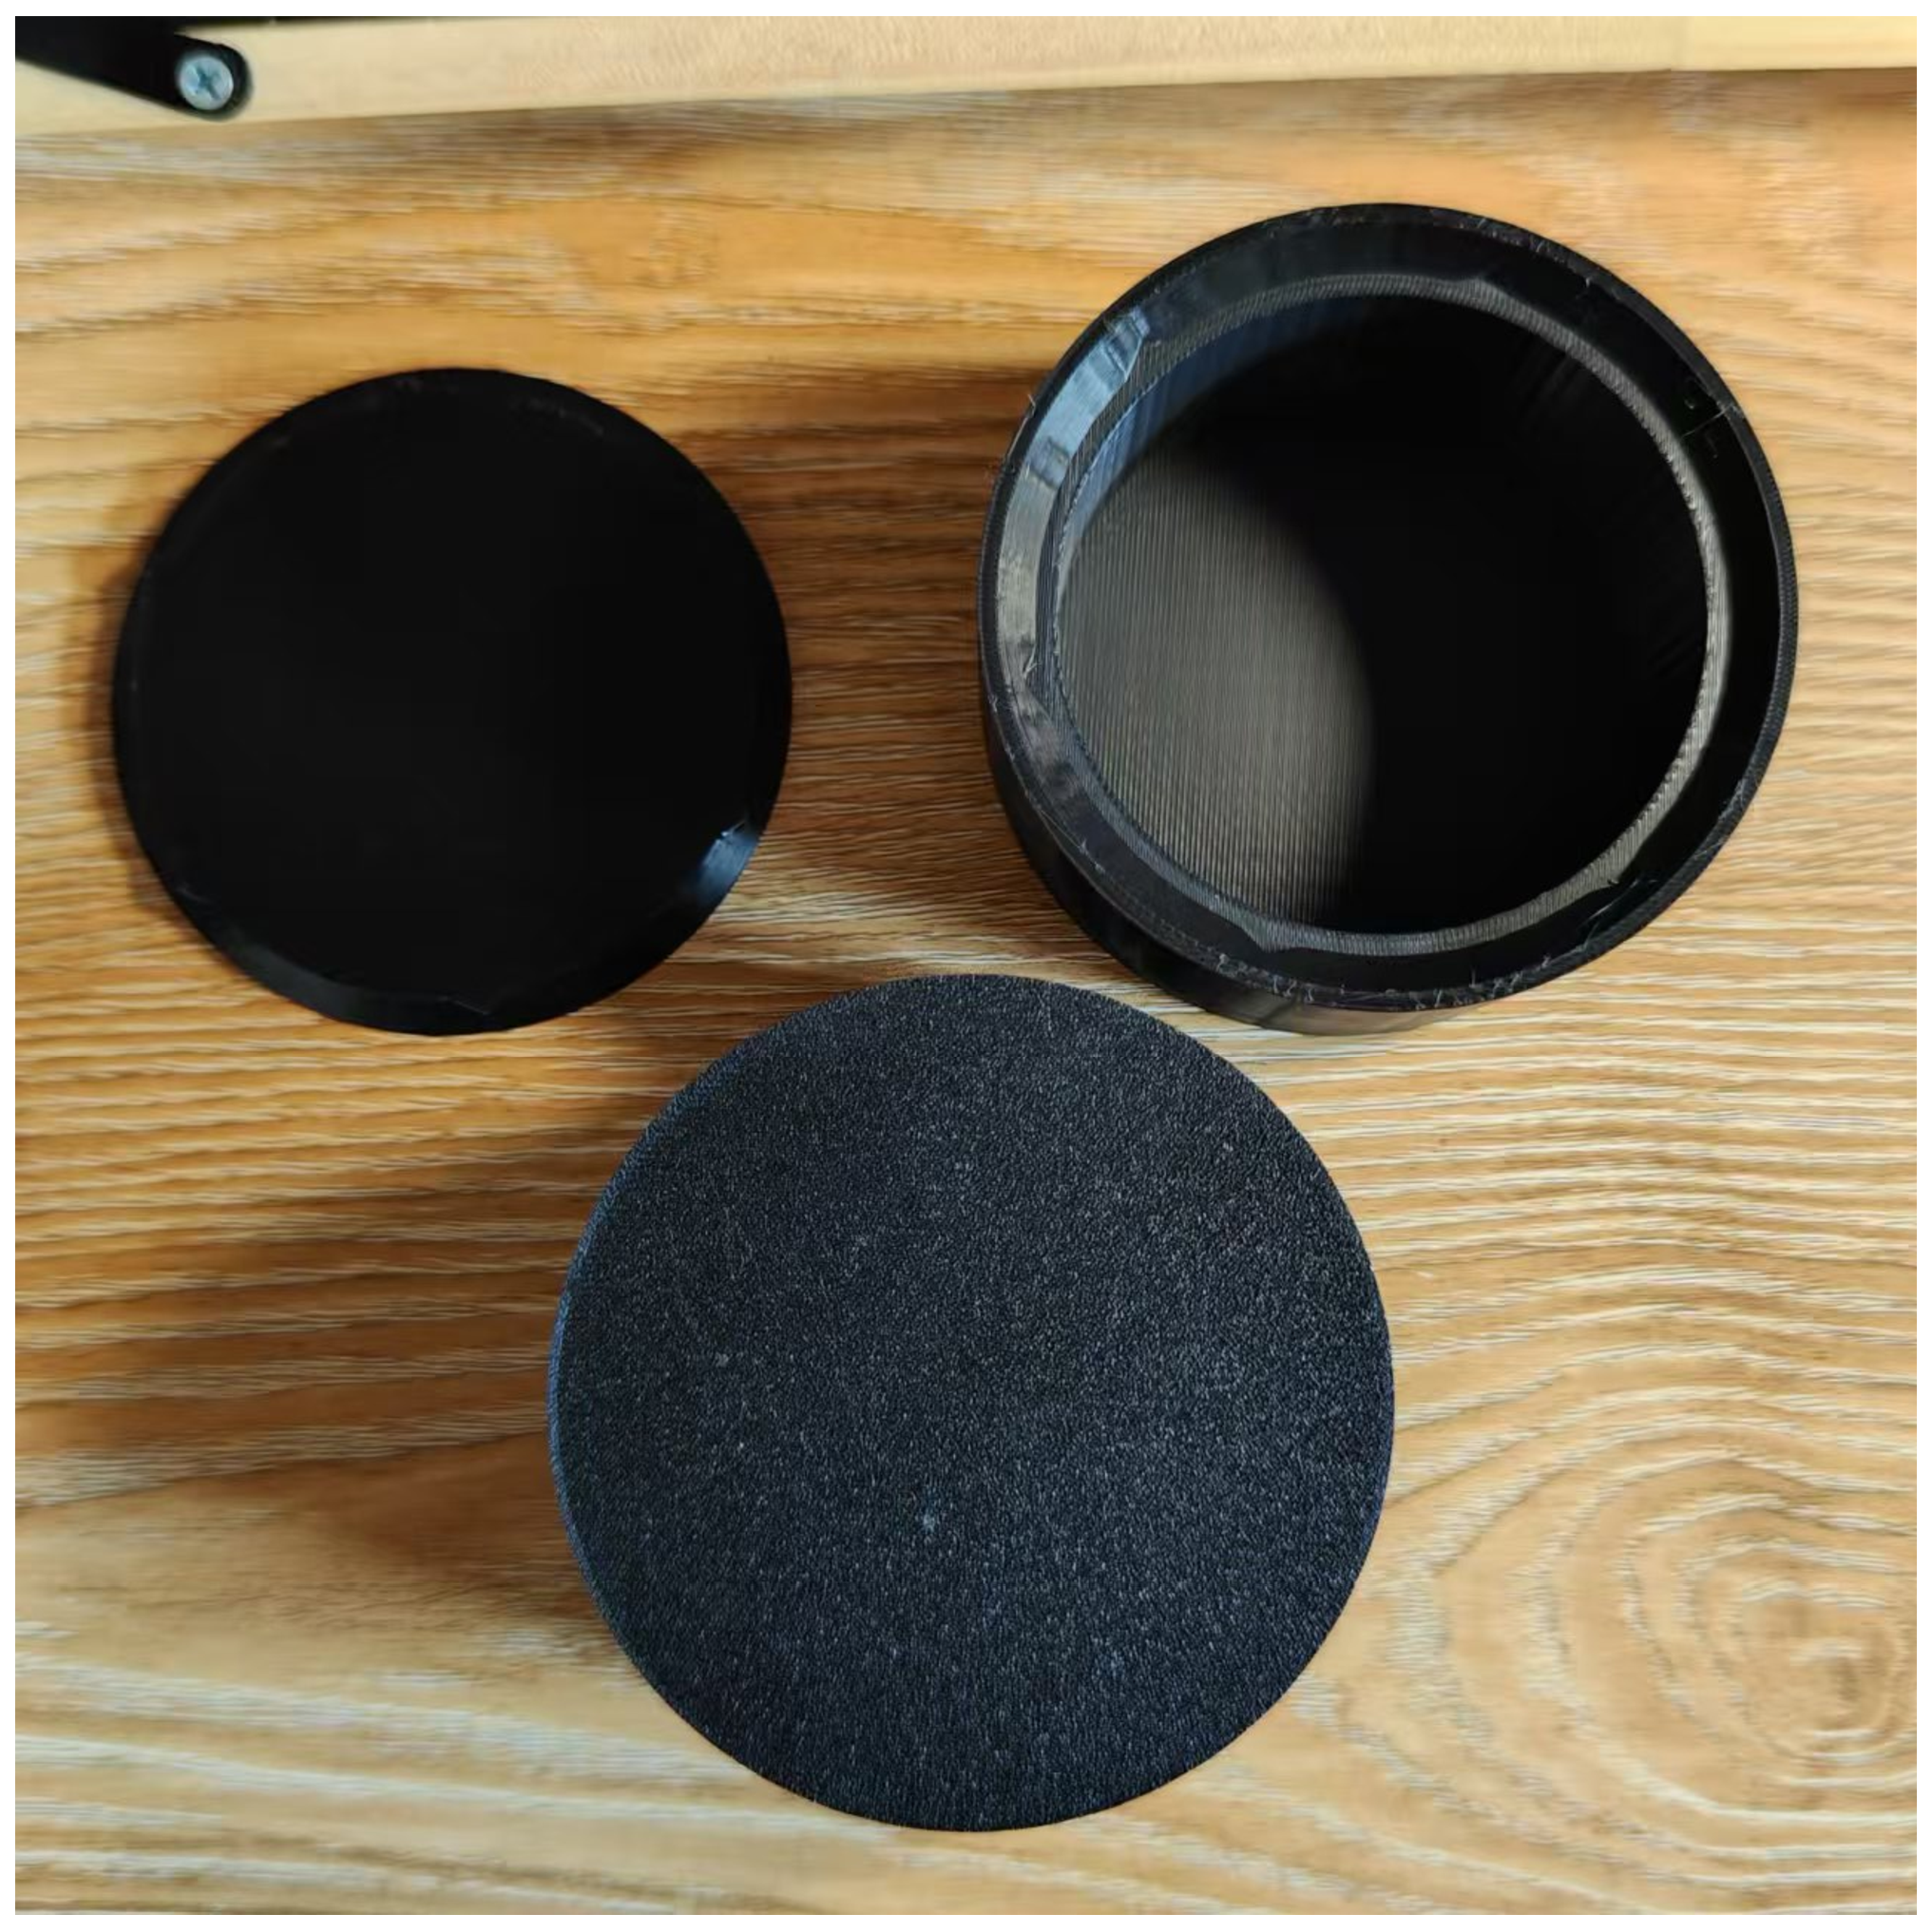
\includegraphics{container.eps}
    \caption{\text{实验容器设备}}
\end{figure}

\begin{table}[h!]
\centering
\begin{tabular}{|c|c|c|c|c|c|c|c|c|}
    \hline
        容器质量/$g$ & 体系质量/$g$ & 液体质量/$g$ & 总体积/$cm^3$ & 容器外高度/$cm$ & 容器内高度/$cm$ & 容器外直径/$cm$ & 容器内直径/$cm$ & 液体体积/$cm^3$ \\
    \hline
        113.500 & 311.040 & 197.540 & 392.699 & 5.000 & 4.000 & 5.000 & 4.000 & 201.062 \\
    \hline
\end{tabular}
\caption{实验体系的静态测量数据}
\end{table}

这样,代入公式立即求得体系转动惯量:

$$ I_{容器} = I_{侧壁} + 2I_{盖子} = 8.795 \times 10^{-6} N·m^2 $$
$$ I_{液体} = \rho · 2\pi · H · \frac{R^4}{4}
           &= 3.782 \times 10^{-4} N·m^2 $$
$$ I_{总体} = I_{容器} + I_{液体} = 3.870 \times 10^{-4} m^2 $$

在测量液体的转动惯量时,为使得包络线的形状最准确,我们延长了观察的时间。这样,在包络线上的极值点数量更多,更利于我们的拟合。
在测量液体的转动惯量前,我们还对扭丝的扭转常数进行了修正。其结果已在前面呈现过。

为了提取实际实验中的时间-角速度数据,我们编写了一段Python脚本:

\begin{lstlisting}[language=Python]
import os
import numpy as np
import matplotlib.pyplot as plt
from scipy.optimize import curve_fit

# 输入:传感器记录文件,xxx.txt
# 输出:该文件记录的周期,运动图像处于y>0的包络线

# 定义m和n的值

def rdfile(filename):
    # 勿动m n
    m = 1  # 第m个元素的索引(从0开始)
    n = 8  # 第n个元素的索引(从0开始)

    # 检查文件是否以.txt结尾
    if not filename.endswith('.txt'):
        filename += '.txt'

    # 构造完整的文件路径
    file_path = os.path.join('.', filename)
    
    # 初始化一个空列表来存储当前文件的二元组
    file_tuples = []
    
    # 打开文件并按行读取内容
    # print(file_path)
    with open(file_path, 'r', encoding='utf-8') as file:
        for line in file:
            # 移除行尾的换行符并分割行
            elements = line.strip().split()
            
            # 提取第m个和第n个元素,并创建二元组
            if ':' in elements[m][-6:]:
                ind = elements[m][-6:].index(':')
                tmp = (elements[m] + (ind + 1) * '0')[-6:]
            else:
                tmp = elements[m][-6:]
            tuple_ = (tmp, elements[n])
            file_tuples.append(tuple_)
    
    # 将当前文件的二元组列表追加到总列表中
    file_tuples.pop(0)
    file_tuples = list(map(lambda x: (float(x[0]), abs(float(x[1]))), file_tuples))
    print(file_tuples)
    return file_tuples

# 求极值列表
def getT(a: list):
    # 极大值列表
    filtered_elements = [
        a[i] for i in range(1, len(a) - 1)  # 排除列表头尾的元素
        if a[i][1] > a[i - 1][1] and a[i][1] > a[i + 1][1]
    ]

    # 求周期,周期为两个极大值之间的距离乘以2
    Ts = []
    for i in range(1, len(filtered_elements)):
        Ts.append(filtered_elements[i][0] - filtered_elements[i - 1][0])

    # 周期
    return 2 * np.mean(Ts), filtered_elements

# 绘制包络线并拟合其方程
def draw(max_tuple_list: list):

    # 使得数据集单调
    def cmp(o: tuple):
        return o[1]
    
    maximum_of_maximum = max(max_tuple_list, key=cmp)
    max_tuple_list = [
        i for i in max_tuple_list 
        if i[0] >= maximum_of_maximum[0] and i[1] <= maximum_of_maximum[1]
    ]
    x = np.array([point[0] for point in max_tuple_list])
    y = np.array([point[1] for point in max_tuple_list])

    # 定义指数衰减的包络线拟合函数
    def envelope_func(t, omega_0, beta):
        return omega_0 * np.exp(-beta * t)

    # 曲线拟合
    popt, _ = curve_fit(envelope_func, x, y, p0=(max(y), 0.1))  # 初值假设
    omega_0_optimized, beta_optimized = popt

    # 使用拟合参数生成拟合曲线
    y_fit = envelope_func(x, *popt)

    # 绘图
    plt.scatter(x, y, label='Envelope Data', color='blue', alpha=0.6)
    plt.plot(x, y_fit, label=f'Fitted Curve: $\\omega_0={omega_0_optimized:.3f}, \\beta={beta_optimized:.3f}$', color='red', linewidth=2)
    plt.xlabel('Time')
    plt.ylabel('Amplitude')
    plt.title('Damped Oscillation Envelope and Fitting')
    plt.legend()
    plt.grid()
    plt.show()

    # 输出优化参数
    print(f"Optimized Parameters: \u03c9_0={omega_0_optimized:.3f}, \u03b2={beta_optimized:.3f}")

# main
if __name__ == "__main__":
    filename = input("Enter the filename: ")
    data = rdfile(filename)
    period, max_points = getT(data)
    print(f"Detected period: {period}")
    draw(max_points)    
\end{lstlisting}

这段Python脚本直接读取传感器读出的数据,提取其中的时间-角速度对,
分析其周期;提取时间-角速度对中的最大值点,拟合并绘制包络线及其函数参数。

\begin{figure}[htbp]
    \centering
    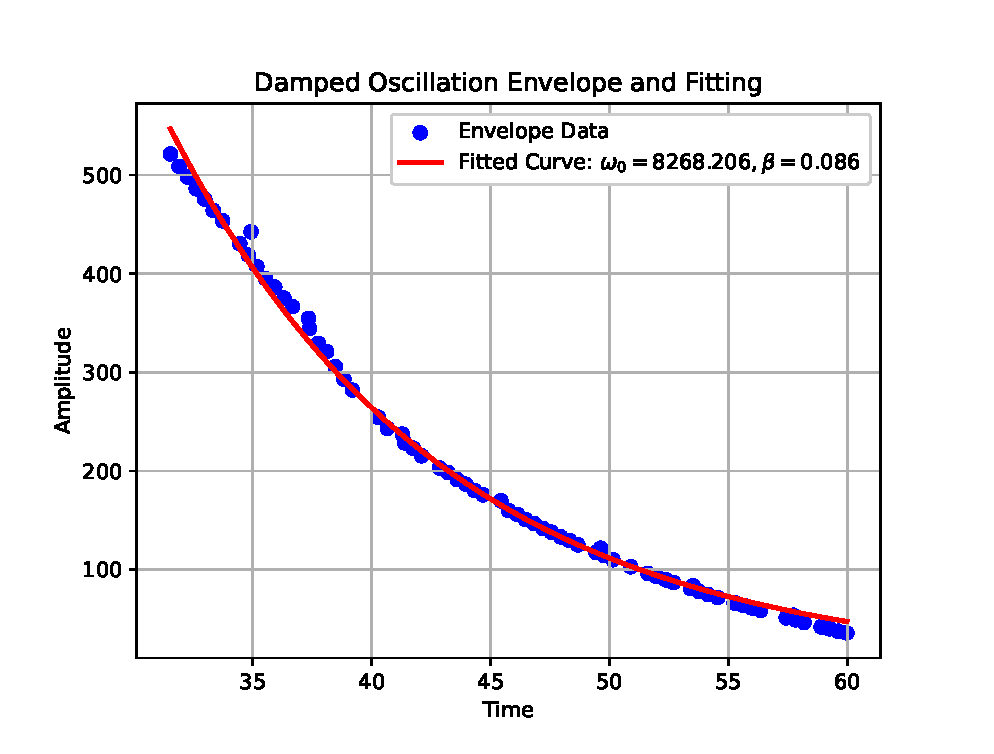
\includegraphics{Figure_1.eps}
    \caption{\text{脚本绘制的时间-角速度图像包络线}}
\end{figure}

我们利用脚本读出$T = 0.783s$,$\omega_0 = 8.020rad/s$。代入公式可得:
$ I_{实验} = 7.464·10^{-5} N·m^2 $,相对误差为$ u = \frac{I_{理论} - I_{实验}}{I_{理论}} \times 100\% = 80.72\% $。

利用脚本,我们还得以读出装有液体的容器做阻尼运动的近似阻尼系数$\beta_1$,为$0.086$。对照组(空容器)读出的阻尼系数$\beta_0$为$0.048$,
我们认为这是作用在器壁外表面的空气阻尼。那么,仅由液体提供的阻尼系数为$ \beta = \beta_1 - \beta_0 = 0.038 $,占$44.19\%$。
作为对照,取计算扭转系数$k$时用以求$T_0$的数据,对标准物体受力进行分析,经过同一脚本处理,
测得空气提供的阻尼系数为$0.018$,证明容器内壁受到的空气阻力不可忽略。

\subsubsection{实验结果}

我们测量了实验扭摆的扭转系数。在较低精度下,其扭转系数为$5.223 \times 10^{-5} N·m^2$;在条件允许的最高精度下,
其扭转系数为$4.806 \times 10^{-5} N·m^2$。
相对误差为$ u = \frac{k_{低} - k_{高}}{k_{高}} \times 100\% = 8.68\% $。

我们使用扭摆法测量了不规则物体的转动惯量。对实验的不规则物体,
其转动惯量为$ I = 9.602 \times 10^{-7} kg·m^2 $。

我们使用扭摆法测量了含有液体的容器的转动惯量,把液体当作刚体对待计算出的体系理论转动惯量$3.870·10^{-4} N·m^2$
与实验测出的体系转动惯量$7.464·10^{-5} N·m^2$相去甚远。
我们还测算了这种运动下装置受到的阻尼,其中由液体贡献的部分占$44.19\%$。
我们猜想,当体系旋转时,仅有贴近容器内壁的薄层液体随容器旋转,
而液体提供的阻尼则是未旋转或未达到与内壁共速的液体对内壁和共速液体提供的阻尼之和。

\begin{figure}[htbp]
    \centering
    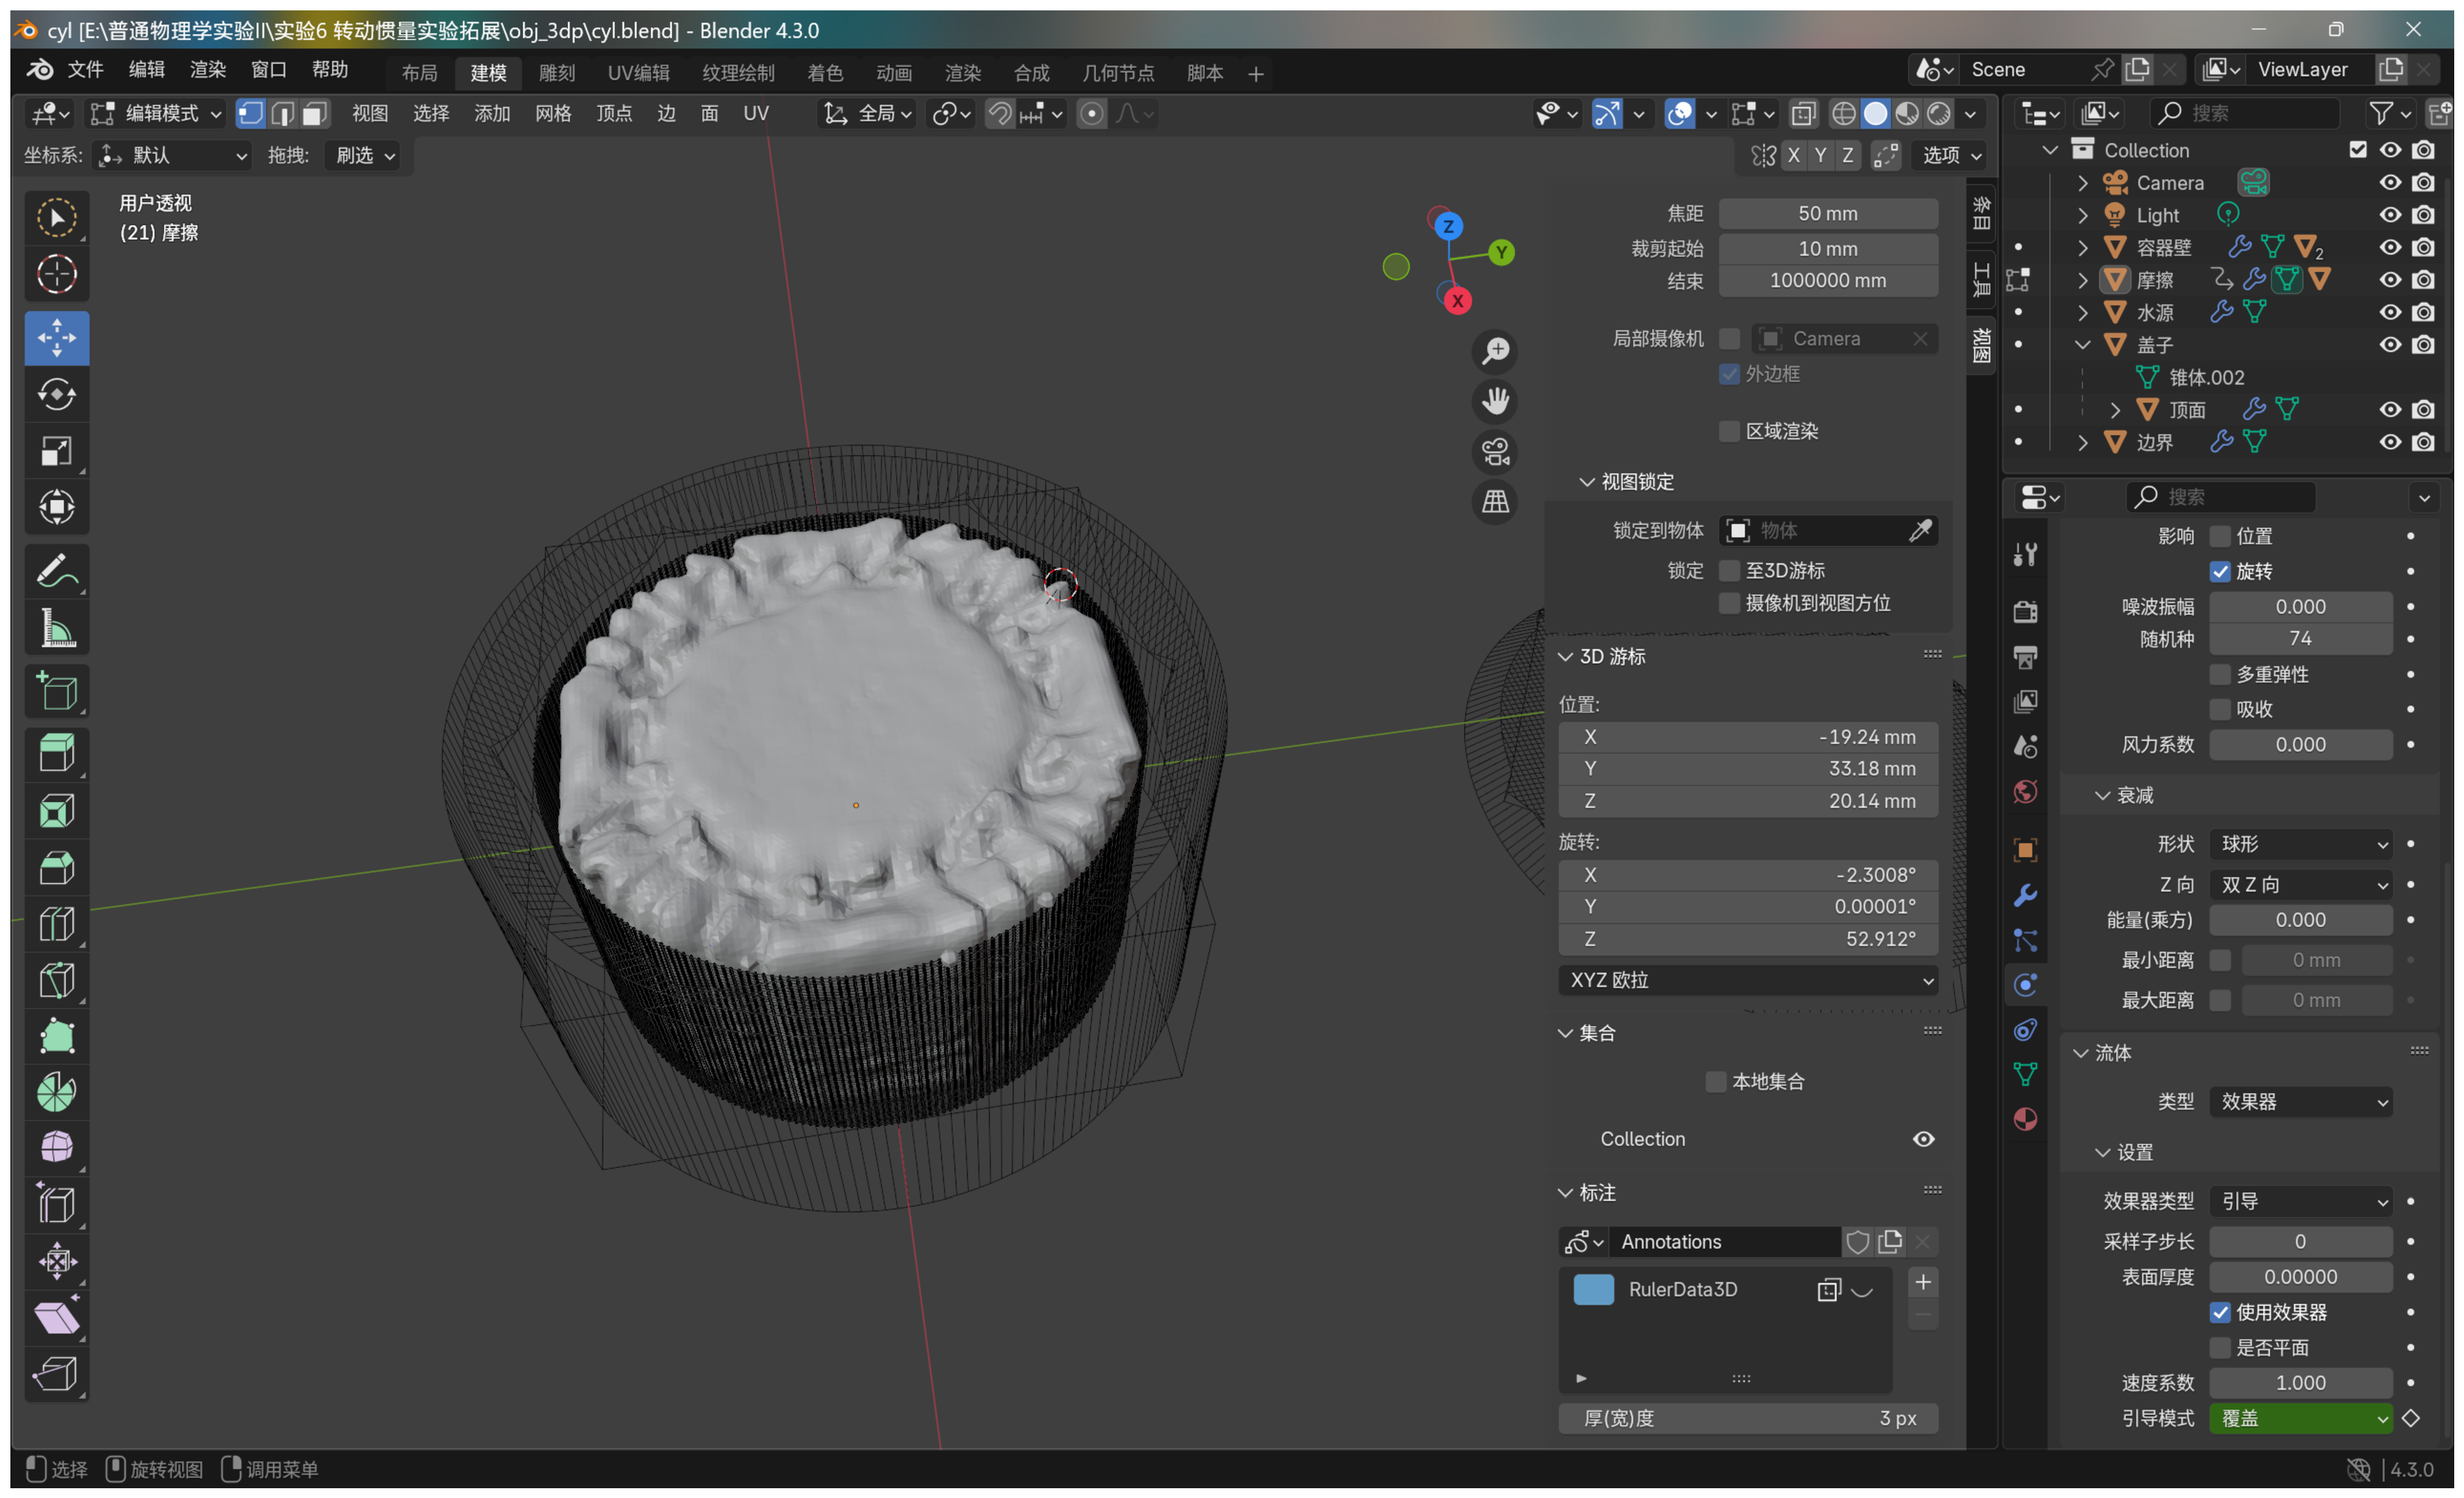
\includegraphics{blender.eps}
    \caption{\text{Blender制作的旋转液体动画}}
\end{figure}

Blender动画也支持这一结果:如图所示,在旋转时,短时间内,仅外层的薄层液体产生了流,
而内层的液体则相对静止。

因此,我们认为,使用刚体转动行为来拟合实验液体——水的转动行为是不合理的。

\subsubsection{误差来源与分析}

\begin{figure}[htbp]
    \centering
    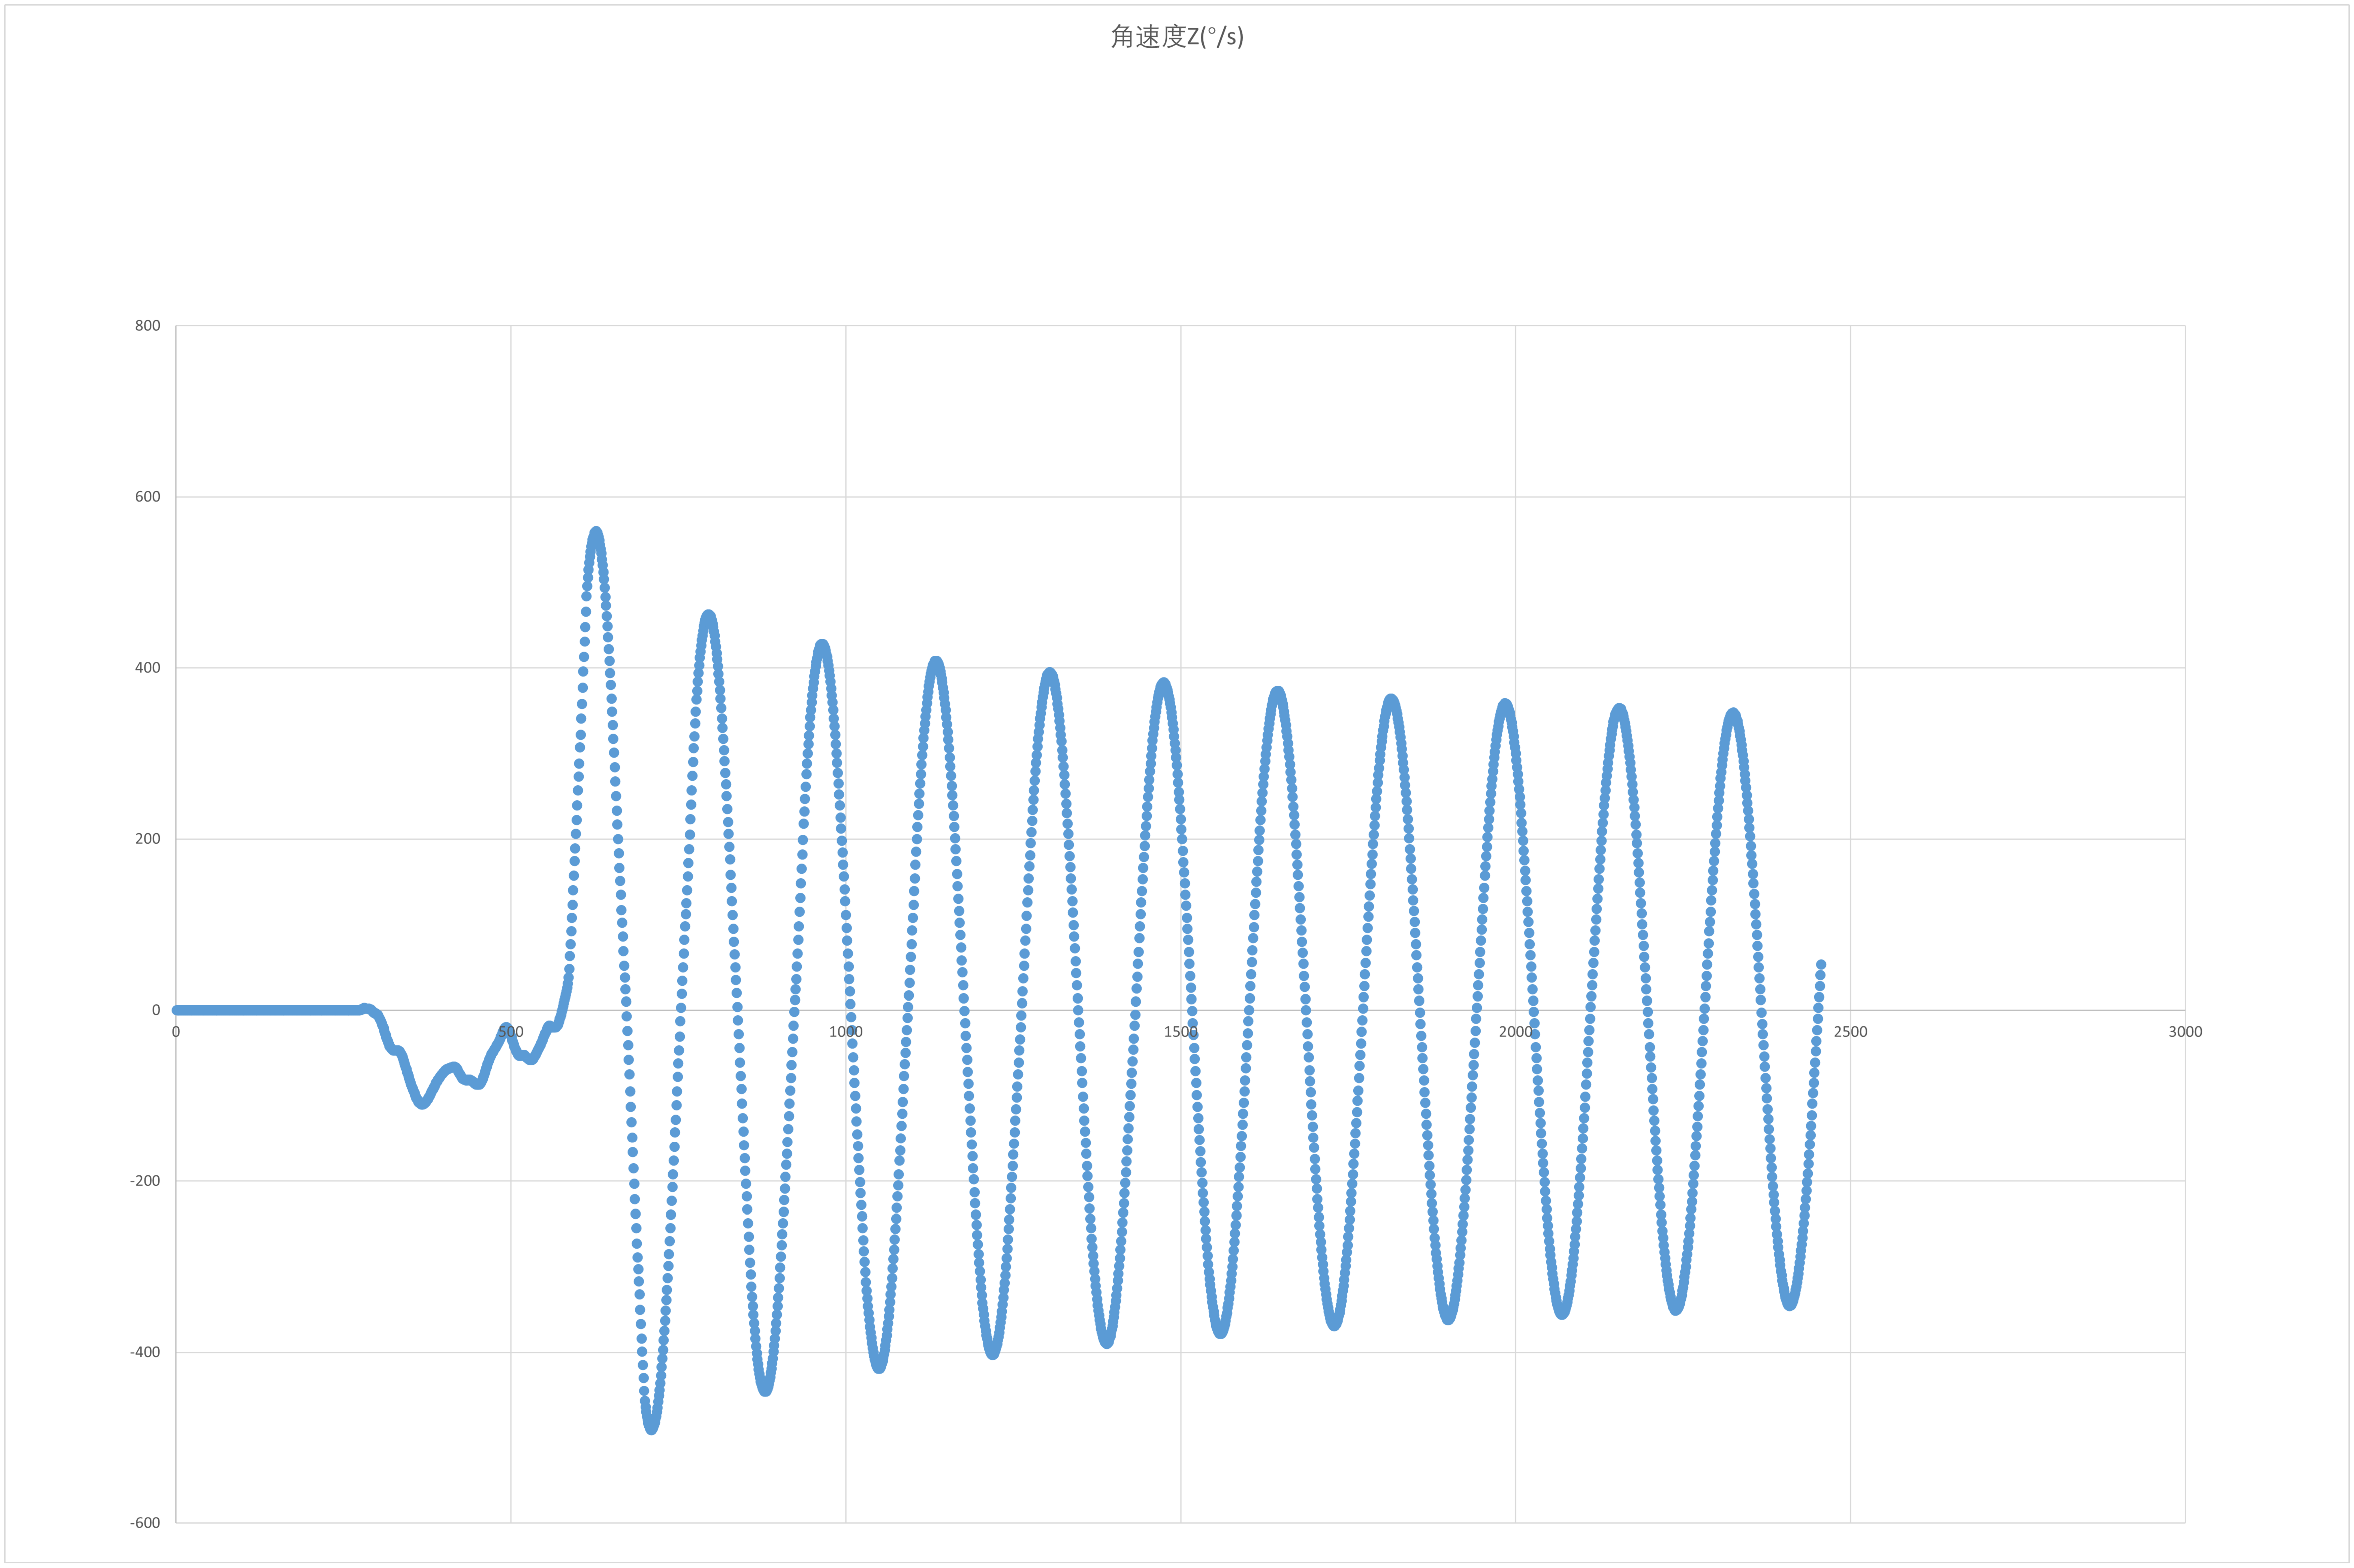
\includegraphics{damp.eps}
    \caption{\text{角速度-时间图像提示阻尼的存在}}
\end{figure}

1. 周期的取样精度

提高周期的取样精度可以提高数学上的精确度。

2. 空气阻力的影响

从传感器上读出的数据可以看出,无论在哪一组实验中,体系都没有做简谐振荡,而是类阻尼振荡。
由于阻尼力的存在,随着体系逐渐接近平衡位置,体系的角速度缓慢减小,周期缓慢增大。
在扭摆法的几个实验中,我们利用自己编写的数据处理程序对阻尼系数进行了简单的定量分析,
测得空气提供的阻尼系数为$0.018$左右;若旋转体具有内壁,则空气提供的阻尼系数增加至$0.048$。
但是,受容器内壁、外壁加工精度限制,其阻尼系数不但由空气影响,还受到侧壁形状的影响。

3. 液体阻尼

液体阻尼在本实验场景中并不是常数,而是由多种阻尼复合的非线性函数。我们将在“拓展:流体力学转动惯量研究”节进行讨论。

\subsection{三线摆法}
\subsubsection{实验方法}

三线摆测量物体转动惯量时,先使下悬盘单独转动,依据$ I = \frac{mRrg}{4 {\pi}^2 H} T^2 $ ,
测出下悬盘的转动周期并代入公式计算,可得下悬盘的转动惯量$I_0$。
在下悬盘上放置待测物体,同样测量转动周期并代入公式计算,可得到下悬盘与待测物体的总转动惯量$I_1$,
$I_1-I_0$即为待测物体的转动惯量。
此外,单独改变某个条件,测量结果的变化趋势,可以探究得到该物理量对于实验结果的影响,
据此可以设计拓展实验。

\subsubsection{实验步骤}

1. 测量下悬盘的转动惯量

(1) 用数字电子称测量三线摆下悬盘的质量,以游标卡尺测出上下悬盘的直径。

(2) 通过三线摆上下悬盘上的水准器,调节螺丝使得上下悬盘保持水平。

(3) 调节上下悬盘之间的距离约为45cm,并测量三线摆上下悬盘之间的间距。

(4) 安装用于测量周期的光电门,使下悬盘在摆动时可以被光电门有效检测到,
设置光电门为记录20个周期的总时间。

(5) 稳定下悬盘,使其不晃动,再轻拨上悬盘,使下悬盘作小角度摆动,
注意不要使下悬盘发生平动。

(6) 用光电门读出下悬盘摆动20个周期所需要的总时间。

(7) 代入公式计算得到下悬盘的转动惯量$ I_0 $。

2. 测量各物体的转动惯量

(1) 准备各个待测物体,包括金属圆环,大圆柱,金属圆筒,
用数字电子称测量各个物体的质量,以游标卡尺测出各个物体的外径和内径。

(2) 把物体置于下悬盘,中心轴和悬盘中心轴重合。

(3) 稳定下悬盘,使其不晃动,再轻拨上悬盘,使下悬盘作小角度摆动。

(4) 用光电门读出下悬盘与待测物体共同摆动20个周期所需要的总时间。

(5) 计算物体和下悬盘总的转动惯量$ I_1 $,物体的转动惯量即为$ I_1 - I_0 $。

3. 验证平行轴定理

(1) 在下悬盘上距圆心3.5cm处的两个对称孔内分别放入相同的的砝码。

(2) 用光电门读出下悬盘与砝码共同摆动20个周期所需要的总时间,计算砝码的转动惯量。

(3) 将两个砝码移至其他孔,距离圆心距离每次增加1cm,重复步骤(2)。

(4) 将计算得到的砝码转动惯量分别除以对应的到圆心距离的平方,看数值是否相近。

4. 探究上圆盘驱动和下圆盘驱动对实验结果的影响

(1) 把金属圆环置于下悬盘,中心轴和悬盘中心轴重合。

(2) 稳定下悬盘,使其不晃动,再轻拨上悬盘,使下悬盘作小角度摆动,
注意不要使下悬盘发生平动。

(3) 用光电门读出下悬盘与金属圆环共同摆动20个周期所需要的总时间,计算金属圆环的转动惯量。

(4) 轻拨下悬盘,使下悬盘作小角度摆动,同样注意不要使下悬盘发生平动,重复步骤(3)。

(5) 将两种驱动方式计算得到的金属圆环的转动惯量进行比较,看数值是否相近。

5. 探究上下悬盘间距对于实验结果的影响

(1) 用米尺测量上下悬盘之间的间距。

(2) 用光电门读出下悬盘与金属圆环共同摆动20个周期所需要的总时间,
计算金属圆环的转动惯量。

(3) 取下金属圆环,改变悬线长度,重新根据水准器调节上下悬盘水平,再次测量上下悬盘之间的间距,
重复步骤(2)。

(4) 查看随上下悬盘间距的变化,所测得的金属圆环的转动惯量如何变化。

6. 探究测量时间选择对数据测量的影响

(1) 把金属圆环置于下悬盘,中心轴和悬盘中心轴重合。

(2) 使用光电门记录每10个摆动周期的时间,共80次 。

(3) 查看随时间的增长,每10个摆动周期的时间是否发生变化。

\subsubsection{实验数据}

1. 测量下悬盘的转动惯量

\begin{table}[h!]
\centering
\begin{tabular}{|c|c|c|c|c|c|}
    \hline
      待测物 & 质量/$kg$ & 周期/$s$ & 转动惯量/$kg·m^2$ & 转动惯量理论值/$kg·m^2$ & 百分误差\\
    \hline
      下悬盘 & 1.322 & 1.262 & 5.996E-03 & 5.901E-03 & 1.61\% \\
    \hline
\end{tabular}
\caption{测量下悬盘的转动惯量}
\end{table}

2. 测量各物体的转动惯量

\begin{table}[h!]
\centering
\begin{tabular}{|c|c|c|c|c|c|c|c|c|c|c|c|}
    \hline
    待测物 & 质量/$kg$ & 周期/$s$ & 转动惯量/$kg·m^2$ & 转动惯量理论值/$kg·m^2$ & 百分误差 \\
    \hline
      金属圆环 & 0.351 & 1.240 &  1.328E-03 & 1.326E-03 & 0.18\% \\
    \hline
      金属圆筒 & 0.669 & 1.151 &  1.524E-03 & 1.567E-03 & 2.74\% \\
    \hline
      大圆柱 & 0.713   & 1.089 &  8.737E-04 & 8.851E-04 & 1.28\% \\
    \hline
\end{tabular}
\caption{测量各物体的转动惯量}
\end{table}
    
3. 验证平行轴定理

\begin{table}[h!]
\centering

\begin{tabular}{|c|c|c|c|c|c|}
    \hline
    待测物 & 质量/$kg$ & 周期/$s$ & 转动惯量/$kg·m^2$ & 转动惯量与距离平方之比/$kg$ \\
    \hline
    平行轴定理(位置11) & 0.238 & 1.191 & 2.986E-04 & 2.44E-05 \\
    \hline
    平行轴定理(位置22) & 0.238 & 1.210 & 5.004E-04 & 2.47E-05 \\
    \hline
    平行轴定理(位置33) & 0.238 & 1.235 & 7.762E-04 & 2.57E-05 \\
    \hline
    平行轴定理(位置44) & 0.238 & 1.258 & 1.031E-03 & 2.44E-05 \\
    \hline
    平行轴定理(位置55) & 0.238 & 1.293 & 1.420E-03 & 2.52E-05 \\
    \hline
    平行轴定理(位置66) & 0.238 & 1.325 & 1.795E-03 & 2.48E-05 \\
    \hline
\end{tabular}
\caption{验证平行轴定理}
\end{table}

4. 探究驱动方式对实验结果的影响(待测物为金属圆环)

\begin{table}[h!]
\centering
\begin{tabular}{|c|c|c|c|c|c|c|c|c|c|c|c|}
      \hline
      驱动方式 & 质量/$kg$ & 周期/$s$ & 转动惯量/$kg·m^2$ & 转动惯量理论值/$kg·m^2$ & 百分误差 \\
      \hline
        上悬盘驱动 & 0.351 & 1.240 &  1.328E-03 & 1.326E-03 & 0.18\% \\
      \hline
        下悬盘驱动 & 0.351 & 1.245 &  1.392E-03 & 1.326E-03 & 4.97\% \\
      \hline
\end{tabular}
\caption{驱动方式对实验结果的影响}
\end{table}

5. 探究上下悬盘间距对于实验结果的影响(待测物为金属圆环)

\begin{table}[h!]
\centering
\begin{tabular}{|c|c|c|c|c|c|c|c|c|c|c|c|}
        \hline
        悬盘间距/$cm$ & 质量/$kg$ & 周期/$s$ & 转动惯量/$kg·m^2$ & 转动惯量理论值/$kg·m^2$ & 百分误差 \\
        \hline
          48.0 & 0.351 & 1.240 &  1.328E-03 & 1.326E-03 & 0.18\% \\
        \hline
          44.8 & 0.351 & 1.196 &  1.308E-03 & 1.326E-03 & 1.32\% \\
        \hline
          40.7 & 0.351 & 1.135 &  1.248E-03 & 1.326E-03 & 5.85\% \\
        \hline
\end{tabular}
\caption{上下悬盘间距对于实验结果的影响}
\end{table}

6. 探究测量时间选择对数据测量的影响(待测物为金属圆环)

\begin{table}[h!]
\centering
\begin{tabular}{|c|c|c|c|c|c|c|c|c|}
    \hline
    周期数 & 1-10 & 11-20 & 21-30 & 31-40 & 41-50 & 51-60 & 61-70 & 71-80 \\
    \hline
    总时间/s & 12.352 & 12.349 & 12.346 & 12.353 & 12.336 & 12.336 & 12.344 & 12.265 \\
    \hline
    百分误差 & / & 0.024\% & 0.049\% & 0.008\% & 0.130\% & 0.130\% & 0.065\% & 0.704\% \\
    \hline
\end{tabular}
\caption{测量时间选择对数据测量的影响}
\end{table}

\subsubsection{实验结果}

通过实验测量,最终成功计算得到了各个待测物体的转动惯量,误差保持在3\%以内,
与预期相符,也说明三线摆法是一种优秀的测量物体转动惯量的方法。

通过移动砝码在下悬盘上的位置,并计算砝码转动惯量与距离平方之比,发现各个位置的该值相近,
相比于位置11处的值误差不超过5\%,也验证了平行轴定理的成立。

实验发现,上悬盘驱动和下悬盘驱动测得的转动惯量都相近于理论值,但下悬盘驱动时的测量值
误差更大,原因在于通过下悬盘驱动时,较难保持下悬盘稳定而不发生平动,从数据中也可以看出,
下悬盘驱动时的平均周期要更大,是由于此时可能会做微小幅度的圆锥摆运动。因此应选择以上悬盘
驱动的方式,来保证测量数据的精确性。

在改变上下悬盘间距时,受限于实验器材,悬盘间距只能改变约$8cm$,在此范围内,观察到
悬盘间距较大时,所测得的转动惯量误差也更小,因此应在允许范围内尽量使用较长的悬线。

实验表明,在不同的测量时间段内,周期时间变化很小,误差不超过1\%,说明三线摆可以在较长时间内
保持周期的变化程度不大,也说明其受空气阻力的影响并不大,
这就为实验中的测量和误差分析提供了方便。

\subsubsection{误差来源与分析}

1. 测量误差

实验中的物理量可以通过增加测量次数来减小误差,但仍有一些物理量存在难以消除且
会对实验结果造成较大影响的误差。由于三线摆的装置设计,使得测量上下悬盘的间距成为了
一个难题,在依赖现有仪器的条件下,可以考虑的改进方法为在上悬盘处放置一个吊锤,
用于判断测量使用的米尺是否真正垂直。此外,由于测量周期所使用的光电门存在读数
漂移,在单个周期内的读数会有较大变化,因此采用读取20个周期的总时间,
依此计算单个周期的平均时间,来减小时间读数误差。

另外,对于R、r、H的测量也应加以规范。R与r应当是悬线点与悬盘中心的距离,而非上下悬盘的真正半径,
H应当是上悬盘的上表面与下悬盘的下表面之间的距离,原因在于推导理论计算公式时,都是以悬线与上下悬盘的
接触点来进行分析,在实际测量时也应遵循此原则。

2. 摆动角度

三线摆法的适用条件为小角度摆动,即假设摆动是微小的简谐振动,若摆动角度过大,
则三线摆法计算转动惯量的公式不再适用,从而引入误差。实际上,在实验过程中,
也难以保证每次的摆角都相近,因此就需要增加测量次数来减小误差。

3. 摆线因素

实验中摆线同样会影响实验结果,一方面,摆线为非理想弹性,其长度可能会在摆动
过程中变化,此外,随振幅不同,其长度同样可能发生变化;另一方面,
摆线的质量虽然通常较小,但是仍会对测量结果产生一定影响,因此应选择刚性较强、质量较轻的摆线材料。

4. 空气阻力

空气阻力和摆线与悬挂点的摩擦力会使得摆动的振幅逐渐减小,
导致摆动周期发生变化,从而影响转动惯量的测量。且空气阻力和摩擦力是不可避免的,
但可以通过减小摆动速度、选择光滑的悬挂点材料以及在真空环境下进行实验来减小其影响。
不过在前面的实验6中已经发现,空气阻力对于实验结果的测量影响实际上十分微弱,
因此可以忽略这一部分的误差。

5. 下悬盘平动

由于在测量过程中,摆动情况由肉眼来观察,若下悬盘发生微小平动也难以被观测到,
然而下悬盘发生平动时会对实验结果造成很大的误差,除了在驱动方式、悬盘间距等方面做出约束,
也应当进一步改进三线摆的装置,如增加观测三线摆平动程度的仪器,以减小误差。


\subsection{落体法}
\subsubsection{实验方法}
\begin{itemize}
    \item \textbf{加速过程}:在外力(如砝码拉力)和摩擦力矩的共同作用下,系统产生角加速度 $\alpha_1$。
    \item \textbf{减速过程}:祛码脱落后,系统仅在摩擦力矩作用下继续转动,产生角加速度 $\alpha_2$。
\end{itemize}

系统的转动惯量 $I$ 通过下式计算:
\begin{equation}
    I = \frac{m r^2 (\alpha_1 + \alpha_2)}{\alpha_1 \alpha_2},
\end{equation}
其中:
\begin{itemize}
    \item $m$:砝码质量;
    \item $r$:塔轮半径;
    \item $\alpha_1$:加速过程的角加速度;
    \item $\alpha_2$:减速过程的角加速度。
\end{itemize}

\subsubsection{实验步骤}
\begin{enumerate}
    \item \textbf{实验准备}
    \begin{itemize}
        \item 调整实验装置,确保水平稳定,减少外部干扰。
        \item 安装待测刚体圆盘与祛码,测量祛码的质量 $m$ 和塔轮的半径 $r$。
    \end{itemize}

    \item \textbf{加速过程测量}
    \begin{itemize}
        \item 挂上砝码,释放系统,系统开始加速转动。
        \item 测量系统完成一定圈数所需的时间 $t_1$。
        \item 计算加速角加速度 $\alpha_1$,公式如下:
        \begin{equation}
            \alpha_1 = \frac{\theta}{t_1^2},
        \end{equation}
        其中 $\theta$ 为角位移。
    \end{itemize}

    \item \textbf{减速过程测量}
    \begin{itemize}
        \item 祛码脱落后,系统在摩擦力矩作用下继续转动。
        \item 测量系统完成相同圈数所需的时间 $t_2$。
        \item 计算减速角加速度 $\alpha_2$,公式如下:
        \begin{equation}
            \alpha_2 = \frac{\theta}{t_2^2}.
        \end{equation}
    \end{itemize}

    \item \textbf{数据处理}
    \begin{itemize}
        \item 将测得的 $\alpha_1$ 和 $\alpha_2$ 代入转动惯量计算公式:
        \begin{equation}
            I = \frac{m r^2 (\alpha_1 + \alpha_2)}{\alpha_1 \alpha_2}.
        \end{equation}
        \item 重复实验多次,取平均值以减少实验误差。
    \end{itemize}
    \end{itemize}
\end{enumerate}

\subsubsection{实验数据}
    \begin{itemize}
        \item \textbf{牵引力不同,半径相同($r=15.37\text{mm}$)}
            \item $m=84.90\text g$
            
                \begin{table}[h!]
                \centering
                \begin{tabular}{cccccc}
                \toprule
                \textbf{周期(转)} & \textbf{1} & \textbf{2} & \textbf{3} & \textbf{4} & \textbf{5} \\
                \midrule
                1  & 1.696 & 1.182 & 1.553 & 1.191 \\
                2  & 1.038 & 0.898 & 1.078 & 0.922 \\
                3  & 0.829 & 0.762 & 0.944 & 0.762 \\
                4  & 0.692 & 0.638 & 0.775 & 0.681 \\
                5  & 0.630 & 0.597 & 0.682 & 0.604 \\
                6  & 0.561 & 0.547 & 0.592 & 0.551 \\
                7  & 0.497 & 0.490 & 0.550 & 0.460 \\
                8  & 0.457 & 0.476 & 0.528 & 0.523 \\
                9  & 0.442 & 0.451 & 0.495 & 0.438 \\
                10 & 0.423 & 0.427 & 0.464 & 0.439 \\
                11 & 0.398 & 0.405 & 0.437 & 0.419 \\
                12 & 0.385 & 0.379 & 0.421 & 0.402 \\
                13 & 0.369 & 0.377 & 0.406 & 0.385 \\
                14 & 0.330 & 0.364 & 0.379 & 0.369 \\
                15 & 0.319 & 0.347 & 0.372 & 0.342 \\
                16 & 0.324 & 0.320 & 0.330 & 0.323 \\
                17 & 0.320 & 0.323 & 0.323 & 0.323 \\
                18 & 0.320 & 0.319 & 0.319 & 0.319 \\
                19 & 0.311 & 0.315 & 0.320 & 0.317 \\
                20 & 0.310 & 0.306 & 0.323 & 0.311 \\
                \midrule
                \textbf{平均值} & 0.53255 & 0.49615 & 0.56455 & 0.504 \\
                \bottomrule
                \end{tabular}
                \caption{落体法数据表1}
                \end{table}

            \item $m=59.86\text g$
                \begin{table}[h!]
                    \centering
                    \begin{tabular}{cccccc}
                    \toprule
                    \textbf{周期(转)} & \textbf{1} & \textbf{2} & \textbf{3} & \textbf{4} & \textbf{5} \\
                    \midrule
                    1  & 1.637 & 1.393 & 1.720 & 2.455 \\
                    2  & 1.134 & 1.056 & 1.197 & 1.315 \\
                    3  & 0.927 & 0.858 & 1.085 & 0.937 \\
                    4  & 0.801 & 0.753 & 0.908 & 0.905 \\
                    5  & 0.705 & 0.701 & 0.805 & 0.765 \\
                    6  & 0.667 & 0.623 & 0.745 & 0.700 \\
                    7  & 0.615 & 0.599 & 0.679 & 0.630 \\
                    8  & 0.558 & 0.560 & 0.552 & 0.603 \\
                    9  & 0.544 & 0.522 & 0.621 & 0.565 \\
                    10 & 0.517 & 0.501 & 0.557 & 0.510 \\
                    11 & 0.495 & 0.485 & 0.513 & 0.507 \\
                    12 & 0.462 & 0.465 & 0.505 & 0.488 \\
                    13 & 0.443 & 0.448 & 0.484 & 0.464 \\
                    14 & 0.440 & 0.431 & 0.466 & 0.436 \\
                    15 & 0.426 & 0.404 & 0.448 & 0.435 \\
                    16 & 0.412 & 0.385 & 0.434 & 0.404 \\
                    17 & 0.392 & 0.387 & 0.404 & 0.400 \\
                    18 & 0.385 & 0.385 & 0.386 & 0.393 \\
                    19 & 0.375 & 0.372 & 0.385 & 0.379 \\
                    20 & 0.369 & 0.341 & 0.386 & 0.373 \\
                    \midrule
                    \textbf{平均值} & 0.6152 & 0.58345 & 0.664 & 0.68285 \\
                    \bottomrule
                    \end{tabular}
                    \caption{落体法数据2}
                    \end{table}

            \item $m=19.83\text g$
                \begin{table}[h!]
                    \centering
                    \begin{tabular}{ccccc}
                    \toprule
                    \textbf{周期(转)} & \textbf{1} & \textbf{2} & \textbf{3} & \textbf{4} \\
                    \midrule
                    1  & 2.718 & 4.065 & 2.753 \\
                    2  & 2.084 & 2.411 & 2.013 \\
                    3  & 1.701 & 1.888 & 1.652 \\
                    4  & 1.481 & 1.622 & 1.440 \\
                    5  & 1.339 & 1.446 & 1.321 \\
                    6  & 1.152 & 1.315 & 1.217 \\
                    7  & 1.177 & 1.209 & 1.115 \\
                    8  & 1.057 & 1.128 & 1.053 \\
                    9  & 1.006 & 1.066 & 1.007 \\
                    10 & 0.943 & 1.006 & 0.882 \\
                    11 & 0.926 & 0.949 & 0.953 \\
                    12 & 0.891 & 0.924 & 0.882 \\
                    13 & 0.862 & 0.889 & 0.834 \\
                    14 & 0.763 & 0.855 & 0.817 \\
                    15 & 0.836 & 0.825 & 0.787 \\
                    16 & 0.772 & 0.782 & 0.767 \\
                    17 & 0.758 & 0.771 & 0.746 \\
                    18 & 0.725 & 0.751 & 0.725 \\
                    19 & 0.712 & 0.734 & 0.705 \\
                    20 & 0.701 & 0.711 & 0.664 \\
                    \midrule
                    \textbf{总和} & 22.604 & 25.347 & 22.335 \\
                    \bottomrule
                    \end{tabular}
                    \caption{落体法数据表3}
                    \end{table}
                    

        \item \textbf{半径不同,牵引力相同($ m=84.90\text g $)}
            \item $r=20.10\text{mm}$
                \begin{table}[h!]
                    \centering
                    \begin{tabular}{ccccc}
                    \toprule
                    \textbf{周期(转)/s} & \textbf{1} & \textbf{2} & \textbf{3} & \textbf{4} \\
                    \midrule
                    1  & 1.193 & 4.194 & 1.433 & 1.280 \\
                    2  & 0.887 & 7.940 & 0.895 & 0.862 \\
                    3  & 0.692 & 2.215 & 0.726 & 0.700 \\
                    4  & 0.577 & 0.980 & 0.639 & 0.580 \\
                    5  & 0.534 & 0.760 & 0.554 & 0.531 \\
                    6  & 0.484 & 0.645 & 0.511 & 0.484 \\
                    7  & 0.428 & 0.576 & 0.454 & 0.425 \\
                    8  & 0.423 & 0.520 & 0.429 & 0.425 \\
                    9  & 0.387 & 0.447 & 0.413 & 0.382 \\
                    10 & 0.375 & 0.434 & 0.390 & 0.380 \\
                    11 & 0.363 & 0.418 & 0.372 & 0.358 \\
                    12 & 0.332 & 0.390 & 0.335 & 0.338 \\
                    13 & 0.320 & 0.377 & 0.316 & 0.315 \\
                    14 & 0.322 & 0.360 & 0.322 & 0.323 \\
                    15 & 0.301 & 0.339 & 0.316 & 0.321 \\
                    16 & 0.265 & 0.317 & 0.275 & 0.293 \\
                    17 & 0.327 & 0.317 & 0.275 & 0.293 \\
                    \bottomrule
                    \end{tabular}
                    \caption{实验周期数据表4}
                    \end{table}
                    
            \item $r=25.61\text{mm}$
            \begin{table}[h!]
                \centering
                \begin{tabular}{cccc}
                \toprule
                \textbf{周期(转)/s} & \textbf{1} & \textbf{2} & \textbf{3} \\
                \midrule
                1  & 0.949 & 1.885 & 0.957 \\
                2  & 0.642 & 0.878 & 0.708 \\
                3  & 0.621 & 0.664 & 0.586 \\
                4  & 0.515 & 0.559 & 0.484 \\
                5  & 0.464 & 0.501 & 0.464 \\
                6  & 0.426 & 0.443 & 0.426 \\
                7  & 0.393 & 0.419 & 0.381 \\
                8  & 0.373 & 0.378 & 0.373 \\
                9  & 0.349 & 0.368 & 0.348 \\
                10 & 0.335 & 0.318 & 0.336 \\
                11 & 0.320 & 0.315 & 0.313 \\
                12 & 0.306 & 0.312 & 0.305 \\
                13 & 0.272 & 0.302 & 1.501 \\
                \bottomrule
                \end{tabular}
                \caption{实验周期数据表5}
                \end{table}
                
    \end{itemize}

\subsubsection{实验结果}
    \begin{itemize}
        \item \textbf{牵引力不同,半径相同}
            \begin{table}[h!]
                \centering
                \begin{tabular}{cccccc}
                \toprule
                \textbf{砝码质量/g} & \textbf{角加速度/$(\text{s}^{-2})$} & \textbf{转动惯量测定值/$(\text{kg}\cdot \text{m}^2)$} & \textbf{转动惯量理论值/$(\text{kg}\cdot \text{m}^2)$} & \textbf{相对误差} \\
                \midrule
                84.90 & 17.85 & 0.00397 & 0.00394 & 0.99\% \\
                59.86 & 12.17 & 0.00388 & 0.00394 & -1.44\% \\
                19.83 & 3.43 & /          & /          & / \\
                \bottomrule
                \end{tabular}
                \caption{落体法实验结果1}
                \end{table}
                
        \item \textbf{半径不同,牵引力相同}
            \begin{table}[h!]
                \centering
                \begin{tabular}{cccccc}
                \toprule
                \textbf{旋转半径/mm} & \textbf{角加速度/$(\text{s}^{-2})$} & \textbf{转动惯量测定值/$(\text{kg}\cdot \text{m}^2)$} & \textbf{转动惯量理论值/$(\text{kg}\cdot \text{m}^2)$} & \textbf{相对误差} \\
                \midrule
                15.37 & 17.85 & 0.00398 & 0.00394 & 0.99\% \\
                20.10 & 19.53 & 0.00397 & 0.00394 & 0.82\% \\
                25.61 & 23.80 & 0.00381 & 0.00394 & -3.09\% \\
                \bottomrule
                \end{tabular}
                \caption{落体法实验结果2}
                \end{table}
                
    \end{itemize}


\subsubsection{误差来源与分析}
    \begin{itemize}
        \item \textbf{主要误差来源}
        \begin{itemize}
            \item 启动阶段的摩擦力矩变化;
            \item 测量时间误差。
        \end{itemize}
        \item \textbf{误差控制}
        \begin{itemize}
            \item 保持加速和减速过程的转速接近;
            \item 使用高精度计时器记录时间。
        \end{itemize}

\section{拓展:流体力学转动惯量探究}
        \subsection{理论背景:液体在匀速旋转容器中转动惯量的计算}
        \textbf{转动惯量的定义}:对于一个连续质量分布的系统,惯性矩 $I$ 可由以下积分公式给出:  
        $$
        I = \int_V r^2 \,dm
        $$  
        其中$r$是质量元 $dm$ 到旋转轴的距离,$V$ 是物体所占的体积,$dm = \rho \, dV$,其中 $\rho$ 是密度,$dV$ 是体积元。
        
        \subsubsection{液体在旋转容器中的建模方法}
        
        假设条件为:容器是一个理想的刚性结构,且绕特定轴旋转。液体的自由表面在旋转时形成稳定的抛物面形状。液体的密度 $\rho$ 是均匀的。
        
        从《普通物理学实验1(H)》课程的“液体旋转实验”中,我们已经知道,液体自由表面的高度分布为: 
        $$
        h(r) = h_0 + \frac{\omega^2 r^2}{2g}
        $$  
        
        其中$h_0$是液体中心的高度,$\omega$ 是角速度,$g$ 是重力加速度,$r$ 是到旋转轴的径向距离。
        
        \subsubsection{惯性矩的计算}
        
        液体的惯性矩 $I$ 表示为:  
        $$
        I = \int_V r^2 \rho \, dV
        $$  
        其中:  
        $$
        dV = r \, dr \, d\theta \, dz
        $$  
        代入惯性矩公式:  
        $$
        I = \rho \int_0^{2\pi} \int_0^{R} \int_0^{h(r)} r^2 \cdot r \, dz \, dr \, d\theta
        $$  
        其中 $R$ 是容器的最大半径,$h(r)$ 是自由表面的高度。
        
        \subsubsection{积分求解}
        \begin{enumerate}
        \item \textbf{对 $z$ 积分}:  
        $$
        \int_0^{h(r)} dz = h(r)
        $$  
        
        代入,得到:  
        $$
        I = \rho \int_0^{2\pi} \int_0^{R} r^3 h(r) \, dr \, d\theta
        $$  
        
        \item \textbf{将 $h(r)$ 代入}:  
        $$
        h(r) = h_0 + \frac{\omega^2 r^2}{2g}
        $$  
        因此:  
        $$
        I = \rho \int_0^{2\pi} \int_0^{R} r^3 \left( h_0 + \frac{\omega^2 r^2}{2g} \right) \, dr \, d\theta
        $$  
        
        \item \textbf{分解积分}:  
        $$
        I = \rho \int_0^{2\pi} d\theta \left[ \int_0^{R} r^3 h_0 \, dr + \int_0^{R} r^3 \frac{\omega^2 r^2}{2g} \, dr \right]
        $$  
        
        \item \textbf{计算径向积分}:  
        对于 $\int_0^R r^3 \, dr$ 和 $\int_0^R r^5 \, dr$,我们分别得到:  
        $$
        \int_0^R r^3 \, dr = \frac{R^4}{4}, \quad \int_0^R r^5 \, dr = \frac{R^6}{6}
        $$  
        将结果代回:  
        $$
        I = \rho \cdot 2\pi \left[ h_0 \cdot \frac{R^4}{4} + \frac{\omega^2}{2g} \cdot \frac{R^6}{6} \right]
        $$  
        
        \item \textbf{化简最终结果}:  
        $$
        I = \frac{\pi \rho R^4 h_0}{2} + \frac{\pi \rho \omega^2 R^6}{6g}
        $$  
        得到我们最终理论推导的式子,即旋转液体转动惯量和转动容器半径、角速度的关系。
        \end{enumerate}

        \subsection{理论比较与误差分析}
        Dodge [2]、Ibrahim [5]、Faltinsen 与 Timokha [6] 对液体阻尼的相关问题进行了全面而系统的阐述,  
        归纳容器内液体的阻尼来自于四个方面:
        1. 液体与容器固壁之间的边界层摩擦阻尼;
        2. 液体内涡的黏性阻尼;
        3. 自由表面阻尼;
        4. 其他三维阻尼。
        
        一般认为液体与容器固壁之间的边界层阻尼是主要作用。  
        对于小幅液体晃动而言,可采用无阻尼不可压缩的势流理论来研究液体晃动,采用速度势的数学模型来描述液体运动,从而可以得到液体的运动方程:
        
        \begin{equation}
        \dot{q_j} + \omega_j^2 q_j = f_j(t), \quad (j = 1, 2, 3, \dots)
        \end{equation}
        
        式中,$q_j$ 为液体系统的第 $j$ 阶自然频率,$\omega_j$ 为第 $j$ 阶固有频率,$f_j(t)$ 为第 $j$ 阶外力。  
        方程(1) 表示了一个无阻尼液体系统的强迫振动方程。当需要考虑液体的晃动阻尼时,可在方程(1)上增加一个阻尼项 $2\zeta_j\omega_j \dot{q_j}$,即有:
        
        \begin{equation}
        \dot{q_j} + 2\zeta_j\omega_j\dot{q_j} + \omega_j^2 q_j = f_j(t), \quad (j = 1, 2, 3, \dots)
        \end{equation}
        
        式中,$\zeta_j$ 为第 $j$ 阶模态的阻尼比系数,主要由阻尼的晃动可以由公式(3)来确定。  
        这种液体晃动阻尼可以通过边界层理论的边界层阻尼来分析。基于 Stokes 边界层理论,可得到容器的边界层阻尼的估计公式为:
        
        \begin{equation}
        \zeta_b = \frac{1}{2} \sqrt{\frac{\nu}{2\omega}} \frac{\int_{\partial S} |\nabla \varphi|^2 ds}{\int_{\int V} |\nabla \varphi|^2 dv}
        \end{equation}
        
        式中:
        - $V$ 为液体空间区域;
        - $\partial S$ 为容器的边界;
        - $\varphi$ 表示了速度势的幅值函数;
        - $\nu$ 为液体运动黏度;
        - $\omega$ 为液体晃动圆频率。
        
        液体内涡的黏性阻尼比可以采用下列黏滞参数计算[6]:
        
        \begin{equation}
        \zeta_v = \frac{\nu}{\omega} \frac{\int_{\int V} \left[ 
        \left(\frac{\partial^2 \varphi}{\partial x^2}\right)^2 + 
        \left(\frac{\partial^2 \varphi}{\partial y^2}\right)^2 + 
        \left(\frac{\partial^2 \varphi}{\partial z^2}\right)^2 + 
        2\left(\frac{\partial^2 \varphi}{\partial x \partial y}\right)^2 + 
        2\left(\frac{\partial^2 \varphi}{\partial y \partial z}\right)^2 + 
        2\left(\frac{\partial^2 \varphi}{\partial z \partial x}\right)^2
        \right] dv}
        {\int_{\int V} |\nabla \varphi|^2 dv}
        \end{equation}
        
        一般认为,以上液体内部的体阻尼比相较于边界层阻尼要小得多,体阻尼可忽略不计。  
        对于短矩形容器,根据公式(3)(4)可得到阻尼比的解析公式。对于非矩形的容器,可采用数值方法计算。

\section{分析与讨论}

\subsection{理论补充}
\subsubsection{基于 LaGrange 方程的建模方法}
假设非线性的转动惯量测定系统具有$n$个广义坐标系,那么其 LaGrange 方程为:
$$ \frac{\text d}{\text dt}(\frac{\partial E}{\partial\overset{.}q_i})-\frac{\partial E}{\partial q_i}+\frac{\partial U}{\partial q_i}=Q_i $$
其中$n$为系统的自由度数目,$q_i$为第$i$个广义坐标,$E$为系统的动能,$U$为系统的势能,$Q_i$为与广义坐标$q_i$对应的广义力,包括阻尼和外加激振力。
取扭摆角$\theta$为广义坐标,代入 LaGrange 方程可得:
$$ \frac{\text d}{\text dt}(\frac{\partial E}{\partial\overset{.}\theta})-\frac{\partial E}{\partial \theta}+\frac{\partial U}{\partial \theta}=Q $$

若系统中的非线性因素是弱的,则微分方程可以表示为:
$$ \overset{..}\theta+\omega_0^2\theta=\varepsilon f(\theta,\overset{.}\theta) $$
其中,$\varepsilon$是小参数,$f(\theta,\overset{.}\theta)$是$\theta,\overset{.}\theta$的非线性解析函数。

该方程的解可以表示为:
$$ \theta=a(t)\cos[\omega_0t+\phi(t)] $$
即把振幅和相位看成时间$t$的函数。该方法称为慢变参数法。
\subsubsection{Runge-Kutta 法}
\subsubsection*{Runge-Kutta法简要介绍}

Runge-Kutta法(简称RK法)是一类用于数值求解常微分方程初值问题的重要算法。它通过引入多步逼近技术,在提高数值解精度的同时保持较高的计算效率,被广泛应用于科学与工程计算中,对于上文提及的 LaGrange 建模方法具有借鉴意义。

\paragraph{问题形式}
Runge-Kutta法主要用于求解以下形式的初值问题:
\[
\frac{dy}{dx} = f(x, y), \quad y(x_0) = y_0,
\]
其中,\( f(x, y) \) 是已知函数,\( y(x) \) 是待求解的函数。

\paragraph{基本思想}
RK方法通过在每一步内结合多个点的斜率(即 \( f(x, y) \) 的值)来计算步进,从而提高解的精度。最简单的RK方法(如欧拉法)只利用当前点的斜率,而高阶RK方法(如经典的四阶Runge-Kutta方法)会结合多个中间点的信息。

\paragraph{经典的四阶Runge-Kutta方法}
四阶Runge-Kutta法是最常用的RK方法之一,其公式为:
\[
k_1 = h f(x_n, y_n),
\]
\[
k_2 = h f\left(x_n + \frac{h}{2}, y_n + \frac{k_1}{2}\right),
\]
\[
k_3 = h f\left(x_n + \frac{h}{2}, y_n + \frac{k_2}{2}\right),
\]
\[
k_4 = h f(x_n + h, y_n + k_3),
\]
\[
y_{n+1} = y_n + \frac{1}{6}(k_1 + 2k_2 + 2k_3 + k_4),
\]
其中:
\begin{itemize}
    \item \( h \) 是步长;
    \item \( k_1, k_2, k_3, k_4 \) 是中间斜率的加权项。
\end{itemize}

该方法利用当前点和三个中间点的斜率估算出下一点的值,具有四阶精度(即局部截断误差为 \( O(h^5) \),全局误差为 \( O(h^4) \))。

\paragraph{总结}
Runge-Kutta法是求解常微分方程的一种高效且精确的方法,其四阶形式因计算精度与效率的良好平衡,在实际应用中极为常见。


\subsection{实验分析}


\subsection{讨论优化}
\subsubsection{实验样件的径向偏移}
根据平行轴定理,径向偏移引起的转动惯量测量误差可以表示为:
$$ \delta=\frac{\pm 2m_AL\Delta L+m_A\Delta L^2}{J_A+m_AL^2} $$

其中$m_A$为实验样件A的质量,$J_A$为实验样件A关于自身中心线的转动惯量。如果$\Delta L<<L$,那么误差公式可以简化为:
$$ -2\frac{\Delta L}{L}<\delta<2\frac{\Delta L}{L} $$
\section{实验总结}
\subsection{实验综述}
在本实验中,小组成员通过探索扭摆法、三线摆法和落体法三种基础的转动惯量测定方法。比较了转动惯量测定方法各自的长处。同时,小组成员利用Blender平台模拟了刚体的转动过程,为今后转动惯量的测定实验提供了一定的参考和借鉴;此外,还利用理论推导与三维建模打印的方法,研究了流体等非刚体旋转时的性质,具有理论探索上的创新性与突破性。
\subsection{不足之处}
    \begin{itemize}
        \item \textbf{三线摆法}
        在三线摆实验部分,实际上还存在许多的改进空间,如探究摆角对于实验结果的影响,在何种摆角范围内会得到最佳的测量条件;另外,实验并没有探究悬盘偏心平动对于实验结果准确度的影响。
        此外,实验也没有对不规则物体的转动惯量进行测量,理论来讲,可以通过悬挂法或者其他方法确定不规则物体的重心,放置于下悬盘的中心轴处就可以测量出该不规则物体的转动惯量,但是由于不规则物体的转动惯量的理论值难以计算,所以最终难以判断测量值与理论值的误差,因此并没有设计这一部分的实验。
    \end{itemize}
\subsection{未来展望}
    受限于实验仪器和实验时间不足,本次实验仍有许多可扩展的空间,期望之后可以引入高精度的计时技术,同时优化摆线材料与测量仪器,并改进测量技术,使实验结果更符合预期。通过不断的技术创新和实验优化,三线摆法将为转动惯量测量领域带来更多的突破与进步。相信在未来,三线摆法不仅将在科研和工程领域中发挥更大的作用,还将在物理教育和跨学科研究中展现出新的潜力。
\section{课题总结}
\subsection{仪器系统照片}

\subsection{实验过程记录}

\subsection{感想}
\begin{itemize}
    \item \textbf{何德怀}
    通过这次为期七周的实验,对于转动惯量的研究方法有了更深刻的认识,此外,对于大型实验的实验设计、进度开展也有了更明确的规划。

\end{itemize}

\section{参考文献}

%%----------- 参考文献 -------------------%%
%在reference.bib文件中填写参考文献,此处自动生成
\reference

\end{document}
